\section{Results}
\label{sec:results}

The results are organised by analysis and linked to the contributions introduced in Section~\ref{sec:introduction}. Primary ensemble discrimination and transfer to unseen sites are reported first, together with comparison to published ABIDE-I studies. The remaining analyses then examine cognitive ability, motion-matched functional-system differences, feature-selection scope, classifier configurations, symptom-severity associations, covariance shrinkage in the windowed representation, probability calibration, and attribution of model scores to functional-system pairs. The feature-selection analysis is treated as a methodological check rather than as one of the five main contributions. Three secondary analyses (confidence-based abstention, combinations of brain parcellations, and label-noise sensitivity) are summarised in one sentence and reported in the Supplementary Material. Throughout, AUROC and accuracy are identified as either participant-pooled estimates or fold means, following Section~\ref{subsubsec:performance-measures}, because these summaries answer different aggregation questions.

\subsection{Classification performance and transfer to unseen sites}
\label{subsec:results-performance}

The highest AUROC of the connectivity-only configurations is obtained with the primary
ensemble under both validation protocols (Table~\ref{tab:configurations}). Specifically, a
fold-mean AUROC of 0.775 is obtained under pooled ten-fold validation, and a fold-mean
AUROC of 0.773 is obtained under LOSO validation. However, the gain over the
best single representation, the windowed tangent mean, is small ($+0.009$ in
participant-pooled AUROC).
Moreover, this gain is not distinguished from chance (unadjusted DeLong $p=0.066$), so it
is not presented as an established improvement. The rank-mean ensemble
(Section~\ref{subsubsec:rank-fusion}) is, in turn, reported for comparison only. Because its score is
not a probability, it has no 0.5 decision threshold, and no accuracy is reported for it.

\begin{table}[pos=htb]
\centering
\caption{Discrimination is evaluated for the ensemble and its individual members in the primary cohort of 871 participants. AUROC and accuracy are reported as fold means, with SD calculated across the outer folds. Because no probability scale is defined for the rank-mean ensemble, accuracy is not reported for this model.}
\label{tab:configurations}
\small
\begin{tabular}{@{}lcccccc@{}}
\toprule
 & \multicolumn{3}{c}{Pooled ten-fold} & \multicolumn{3}{c}{LOSO} \\
\cmidrule(lr){2-4}\cmidrule(l){5-7}
Configuration & AUROC & SD & Accuracy & AUROC & SD & Accuracy \\
\midrule
Ensemble, probability mean (adopted) & 0.775 & 0.040 & 0.707 & 0.773 & 0.087 & 0.684 \\
Windowed tangent, mean & 0.767 & 0.044 & 0.695 & 0.771 & 0.082 & 0.670 \\
Ensemble, rank mean & 0.756 & 0.038 & -- & 0.750 & 0.091 & -- \\
Static tangent & 0.756 & 0.048 & 0.692 & 0.757 & 0.104 & 0.643 \\
Correlation & 0.750 & 0.040 & 0.683 & 0.743 & 0.083 & 0.655 \\
\bottomrule
\end{tabular}
\end{table}

Participant-pooled estimates show similar discrimination under pooled ten-fold and LOSO validation (Table~\ref{tab:performance}; Figure~\ref{fig:performance}a). AUROC is 0.776 under pooled ten-fold validation, with a 95\% DeLong interval of 0.745--0.807, and 0.774 under LOSO validation, with an interval of 0.744--0.805. Under pooled validation, sensitivity and specificity are similar at 0.705 and 0.709, whereas under LOSO validation sensitivity is higher than specificity at 0.742 and 0.684. The LOSO fold-mean accuracy in Table~\ref{tab:configurations} (0.684) is lower than the participant-pooled value in Table~\ref{tab:performance} (0.711) because the former gives equal weight to each of the 20 sites, whereas the latter gives equal weight to each participant; likewise, the LOSO fold-mean AUROC of 0.773 equals the unweighted mean of the 20 site AUROCs, whereas the participant-pooled AUROC is 0.774. Site-clustered bootstrap intervals are wider than the parametric intervals. For pooled validation, the AUROC interval widens to 0.733--0.807 and the accuracy interval to 0.670--0.737, compared with 0.745--0.807 and 0.676--0.736 from DeLong and Wilson intervals. Under LOSO validation, the AUROC interval widens to 0.726--0.808 and the accuracy interval to 0.661--0.748, compared with 0.744--0.805 and 0.680--0.740. The larger change occurs mainly at the lower bounds, but all AUROC intervals remain above 0.5. The choice of penalty strength is also stable to the scope of nesting. When the tangent reference and feature scaler are refitted within every inner split (Section~\ref{subsubsec:nested-penalty}), the selected value changes in only 2 of 30 member fits under pooled validation and 2 of 60 under LOSO validation, with inner-AUROC differences no larger than 0.0004. Participant-pooled AUROC changes from 0.7760 to 0.7756 and from 0.7745 to 0.7746, while accuracy changes from 0.707 to 0.706 and from 0.711 to 0.705. Extending the penalty grid down to $10^{-5}$ still selects 0.001 in 81 of 90 member fits, with AUROCs of 0.7743 and 0.7747. Finally, cohort counts are consistent with the released records. Of 1,112 ABIDE-I phenotypic records, 1,035 have a preprocessed derivative, and 871 meet the three-rater primary rule with usable regional time series, comprising 403 autistic and 468 non-autistic participants. The wider QC cohort is defined by an acceptable functional-image rating from the third rater and contains 1,035 records, of which 1,032 have regional time series. The two 1,035-record sets overlap in 1,033 participants.

\begin{table}[t]
\centering
\caption{Participant-pooled performance of the primary ensemble in the primary cohort
(871 participants), with 95\% intervals. AUROC carries DeLong intervals; accuracy,
sensitivity and specificity carry Wilson intervals.}
\label{tab:performance}
\small
\begin{tabular}{@{}lcccc@{}}
\toprule
Validation & AUROC & Accuracy & Sensitivity & Specificity \\
\midrule
Pooled ten-fold & 0.776 (0.745--0.807) & 0.707 (0.676--0.736) & 0.705 (0.658--0.747) & 0.709 (0.667--0.749) \\
LOSO & 0.774 (0.744--0.805) & 0.711 (0.680--0.740) & 0.742 (0.697--0.782) & 0.684 (0.640--0.724) \\
\bottomrule
\end{tabular}
\end{table}

\begin{figure}[pos=tbp]
\centering
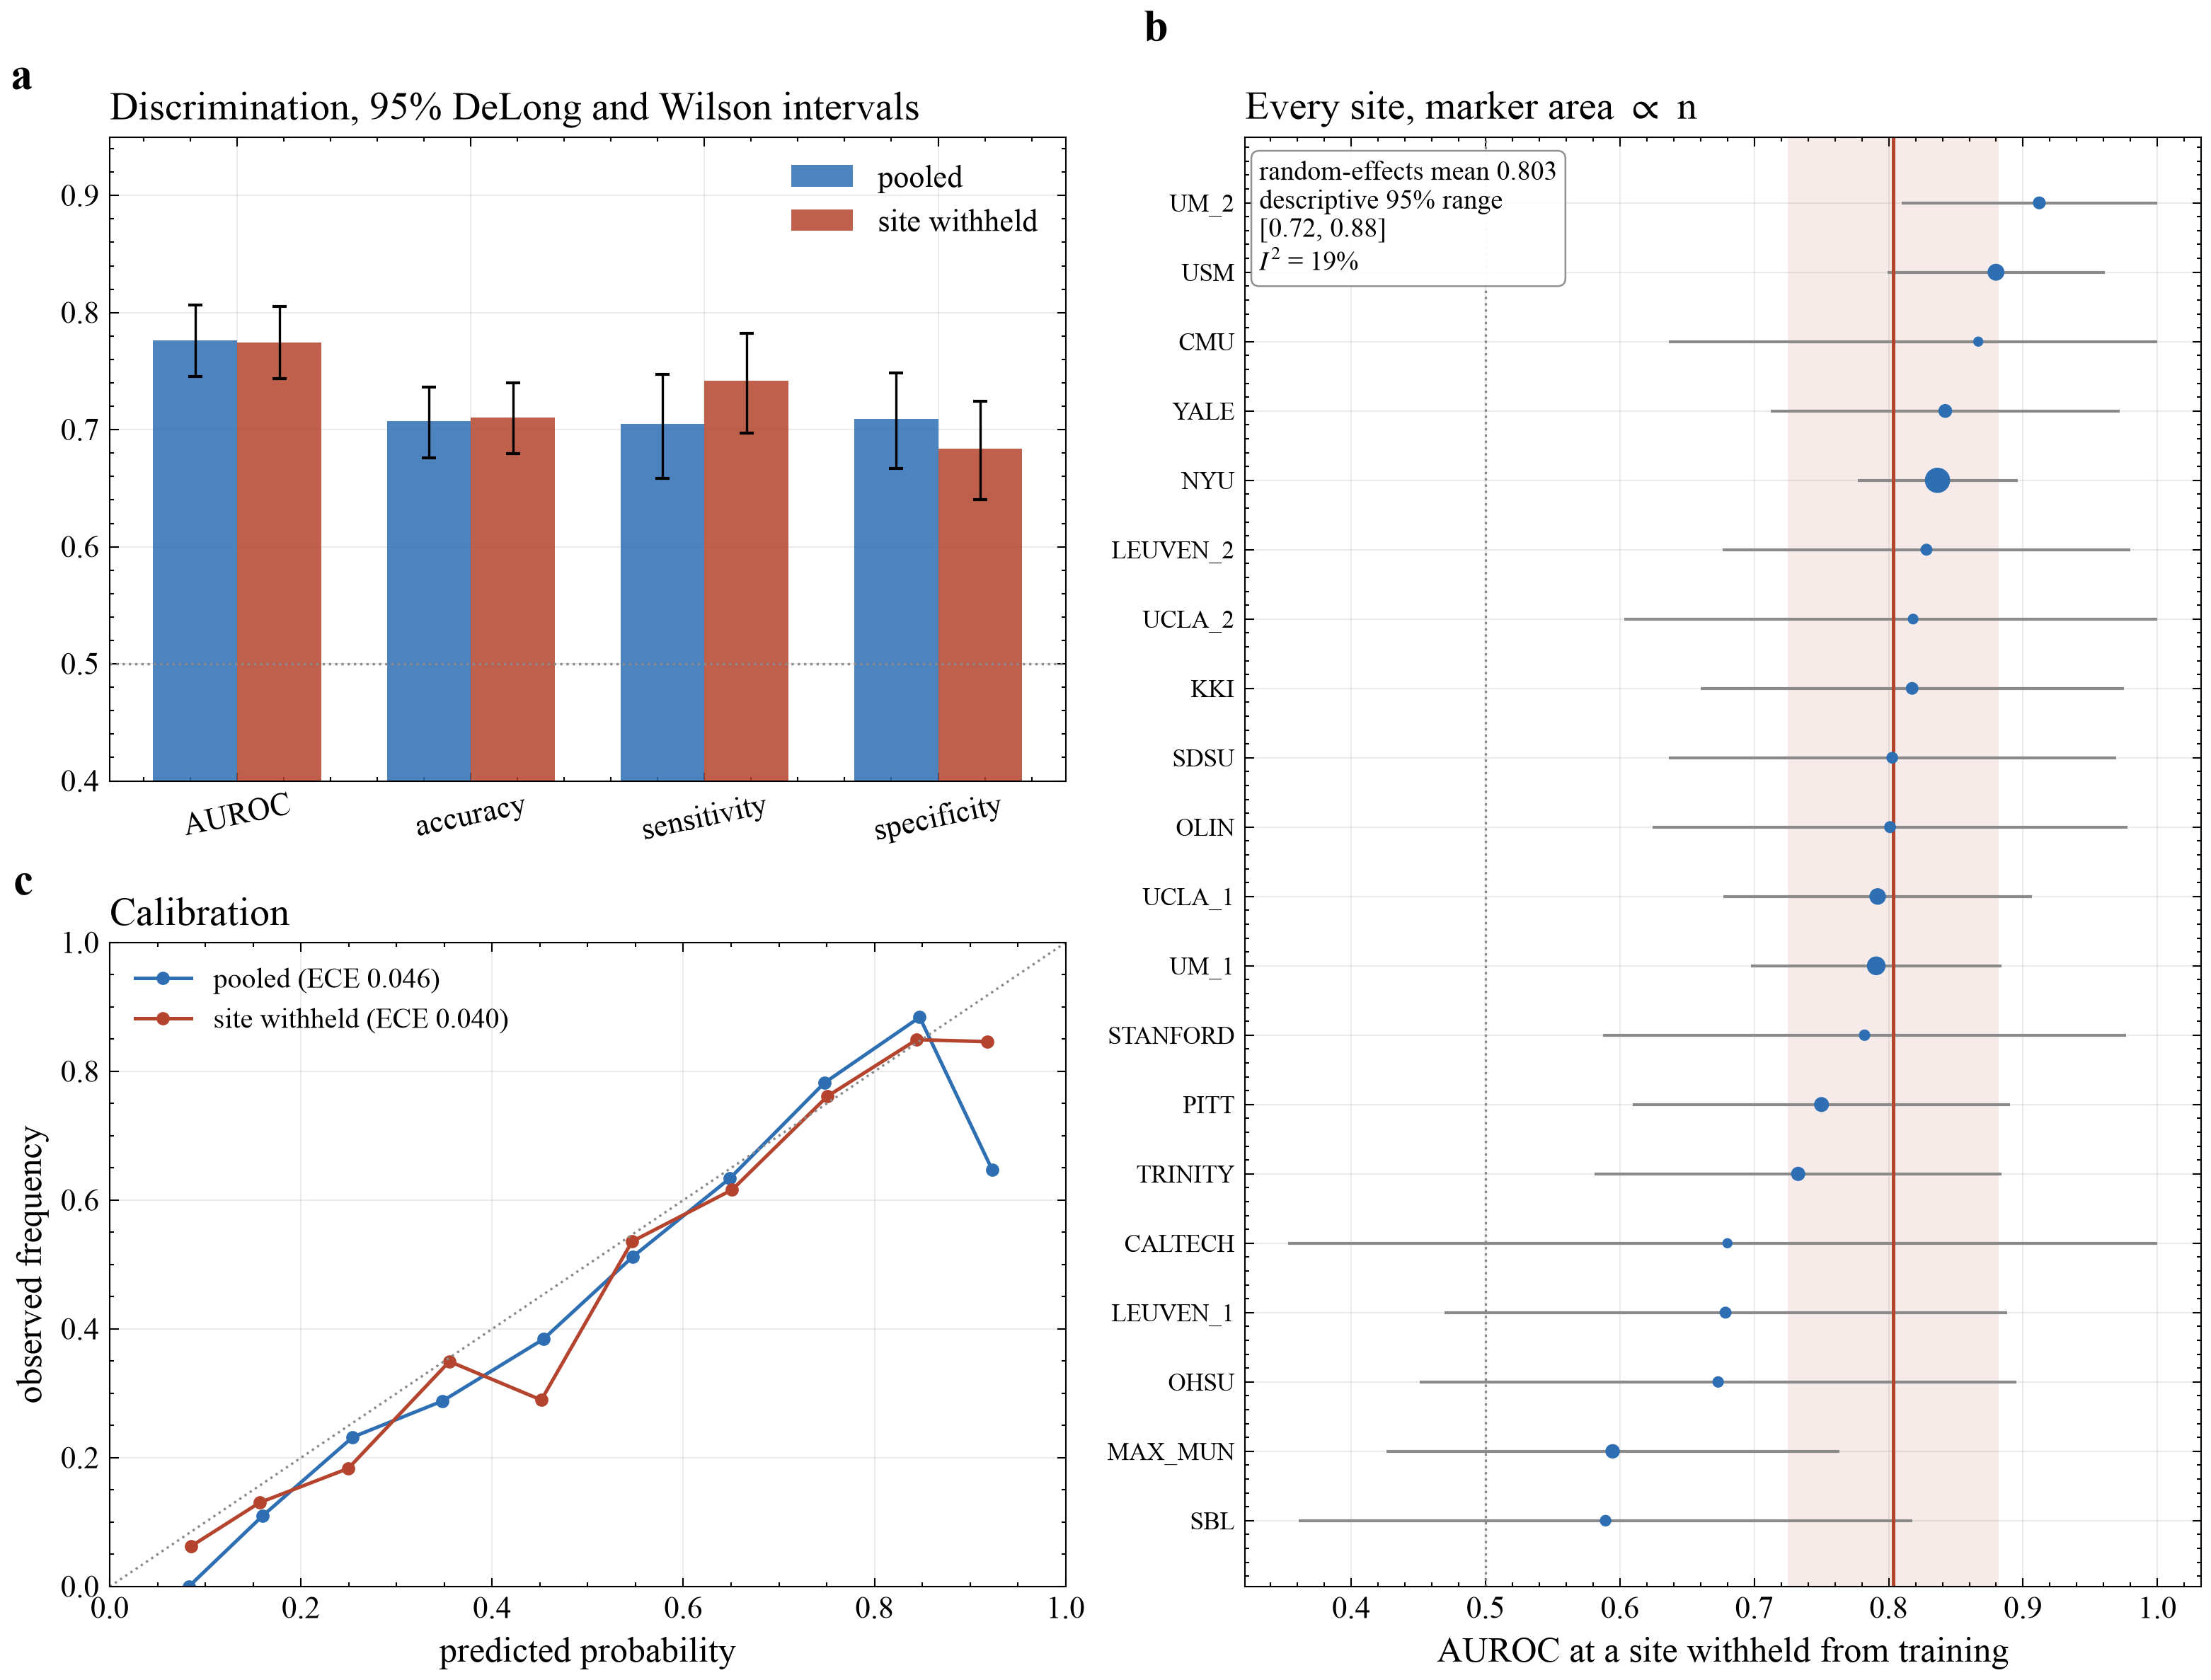
\includegraphics[width=\linewidth]{fig_performance}
\caption{Discrimination, per-site transfer, and calibration of the primary ensemble. (a) Discrimination under both validation protocols, with 95\% DeLong and Wilson intervals reported as lower-bound estimates of uncertainty. (b) AUROC for each site when that site is withheld from training, with marker area proportional to the number of participants. The random-effects mean and the descriptive interval from Equation~\eqref{eq:prediction-interval} are shown; this interval describes the observed sites and is not interpreted as a prediction for an unseen site. (c) Native predicted probabilities against observed frequencies in ten equal-width bins.}
\label{fig:performance}
\end{figure}

\begin{table}[t]
\centering
\caption{Comparison with published ABIDE-I resting-state functional-connectivity studies. Published values are reported as given by the original studies. The present framework additionally reports AUROC under leave-one-site-out validation and probability calibration. n.r., not reported.}
\label{tab:published-comparison}
\small
\setlength{\tabcolsep}{4pt}
\begin{tabular}{@{}>{\raggedright\arraybackslash}p{0.24\linewidth}cccccc@{}}
\toprule
Study & Accuracy & AUROC & Sample & Procedure & AUROC, unseen site & ECE \\
\midrule
\citet{Heinsfeldetal2018} & 0.700 & n.r. & 1,035 & 10-fold & n.r. & n.r. \\
\citet{Eslamietal2019} & 0.703 & n.r. & 1,035 & 10-fold & n.r. & n.r. \\
\citet{AlmuqhimSaeed2021} & 0.708 & n.r. & 1,035 & 10-fold & n.r. & n.r. \\
This work, ensemble & 0.707 & 0.776 & 871 & \reviewdel{nested}\reviewhl{outer} 10-fold & 0.774 ($-0.002$) & 0.046 \\
This work, ensemble, wider QC cohort & 0.706 & 0.789 & 1,032 & \reviewdel{nested}\reviewhl{outer} 10-fold & 0.783 ($-0.006$) & 0.023 \\
This work, tangent model, wider QC cohort & 0.696 & 0.766 & 1,032 & \reviewdel{nested}\reviewhl{outer} 10-fold & -- & -- \\
\bottomrule
\end{tabular}
\end{table}

Variation across acquisition sites is modest despite substantial differences in site size and acquisition conditions. Under LOSO validation, the participant-pooled AUROC is 0.774, only 0.002 below pooled ten-fold validation. Across the 20 withheld sites, AUROC ranges from 0.589 to 0.912, with an unweighted mean of 0.773. A descriptive random-effects model gives a mean AUROC of 0.803 ($Q=23.5$, $p=0.22$; $I^2=19\%$), indicating limited detectable heterogeneity across the observed sites. Because the site-specific estimates share training data and receive unequal statistical weights, this random-effects value is used only to summarise site variation and is not interpreted as an alternative estimate of overall performance. Wider intervals at several sites largely reflect their small sample sizes, with a median of approximately 30 participants per site. Phenotypic variables provide only limited information beyond functional connectivity. A phenotype-only model reaches an AUROC of approximately 0.62, while adding phenotype information to the connectivity ensemble increases participant-pooled AUROC by only 0.004 ($q=0.11$). The phenotype component is therefore not retained in the primary model. This result supports the use of connectivity as the principal source of discrimination in the present framework. For comparison with previous ABIDE-I studies, performance is also evaluated in a wider QC cohort that closely matches their reported eligible sample size as shown in Table~\ref{tab:published-comparison}. After excluding three participants without usable regional time series, 1,032 participants remain. The ensemble achieves a participant-pooled accuracy of 0.706 and an AUROC of 0.789 under pooled ten-fold validation, with a LOSO AUROC of 0.783. The accuracy is directly comparable with previously reported ABIDE-I values of 0.700, 0.703, and 0.708 \citep{Heinsfeldetal2018,Eslamietal2019,AlmuqhimSaeed2021}. These differences are too small to support a claim of numerical superiority. Instead, the present results show that comparable classification accuracy is obtained while additionally using \reviewdel{nested model selection}\reviewhl{outer validation with an inner penalty search}, evaluating transfer to unseen acquisition sites, reporting probability calibration, and avoiding outcome-informed feature selection before cross-validation. Performance changes modestly with cohort definition. The static tangent model reaches a fold-mean AUROC of 0.756 in the primary cohort and 0.766 in the wider QC cohort. Participants included only in the wider cohort have substantially higher mean FD (0.239 versus 0.109 mm), a greater autistic proportion (62.2\% versus 46.3\%), and more frequent rater notes. The two cohorts therefore differ in motion, image-quality characteristics, and diagnostic composition. The AUROC difference \reviewdel{should consequently be interpreted}\reviewhl{is consequently interpreted} as an effect of cohort definition rather than as a change attributable to connectivity alone.

\subsection{Cognitive ability and detection}
\label{subsec:results-cognitive-ability}

Discrimination is lower in the higher-IQ autistic subgroups in the unmatched band analysis, contributing to the fourth study contribution. Because these subgroup analyses are exploratory (Sections~\ref{par:cognitive-sex-subgroups} and~\ref{subsubsec:analysis-status}), the pattern is interpreted descriptively. To keep the comparison group constant, all 468 non-autistic participants are used as the reference for every IQ band, while only autistic participants are divided by full-scale IQ. Under pooled ten-fold validation, AUROC decreases from 0.873 for autistic participants with full-scale IQ below 85 to 0.719 for those with IQ 115 or above (Table~\ref{tab:iq-bands}; Figure~\ref{fig:group-differences}d). A similar pattern is observed under LOSO validation, where AUROC decreases from 0.871 to 0.709. However, the autistic IQ bands still differ from the fixed non-autistic reference group in full-scale IQ, so this unmatched comparison does not isolate IQ from group composition. The matched analysis below addresses this remaining difference.

\begin{table}[t]
\centering
\caption{AUROC by full-scale IQ band of the autistic participants, each band scored
against the same comparison group of all 468 non-autistic participants.}
\label{tab:iq-bands}
\small
\begin{tabular}{@{}lccc@{}}
\toprule
Autistic participants & $n$ & Pooled ten-fold & LOSO \\
\midrule
Full-scale IQ below 85 & 40 & 0.873 & 0.871 \\
Full-scale IQ 85--99 & 97 & 0.815 & 0.816 \\
Full-scale IQ 100--114 & 126 & 0.781 & 0.788 \\
Full-scale IQ 115 or above & 113 & 0.719 & 0.709 \\
\bottomrule
\end{tabular}
\end{table}

\begin{figure}[pos=tbp]
\centering
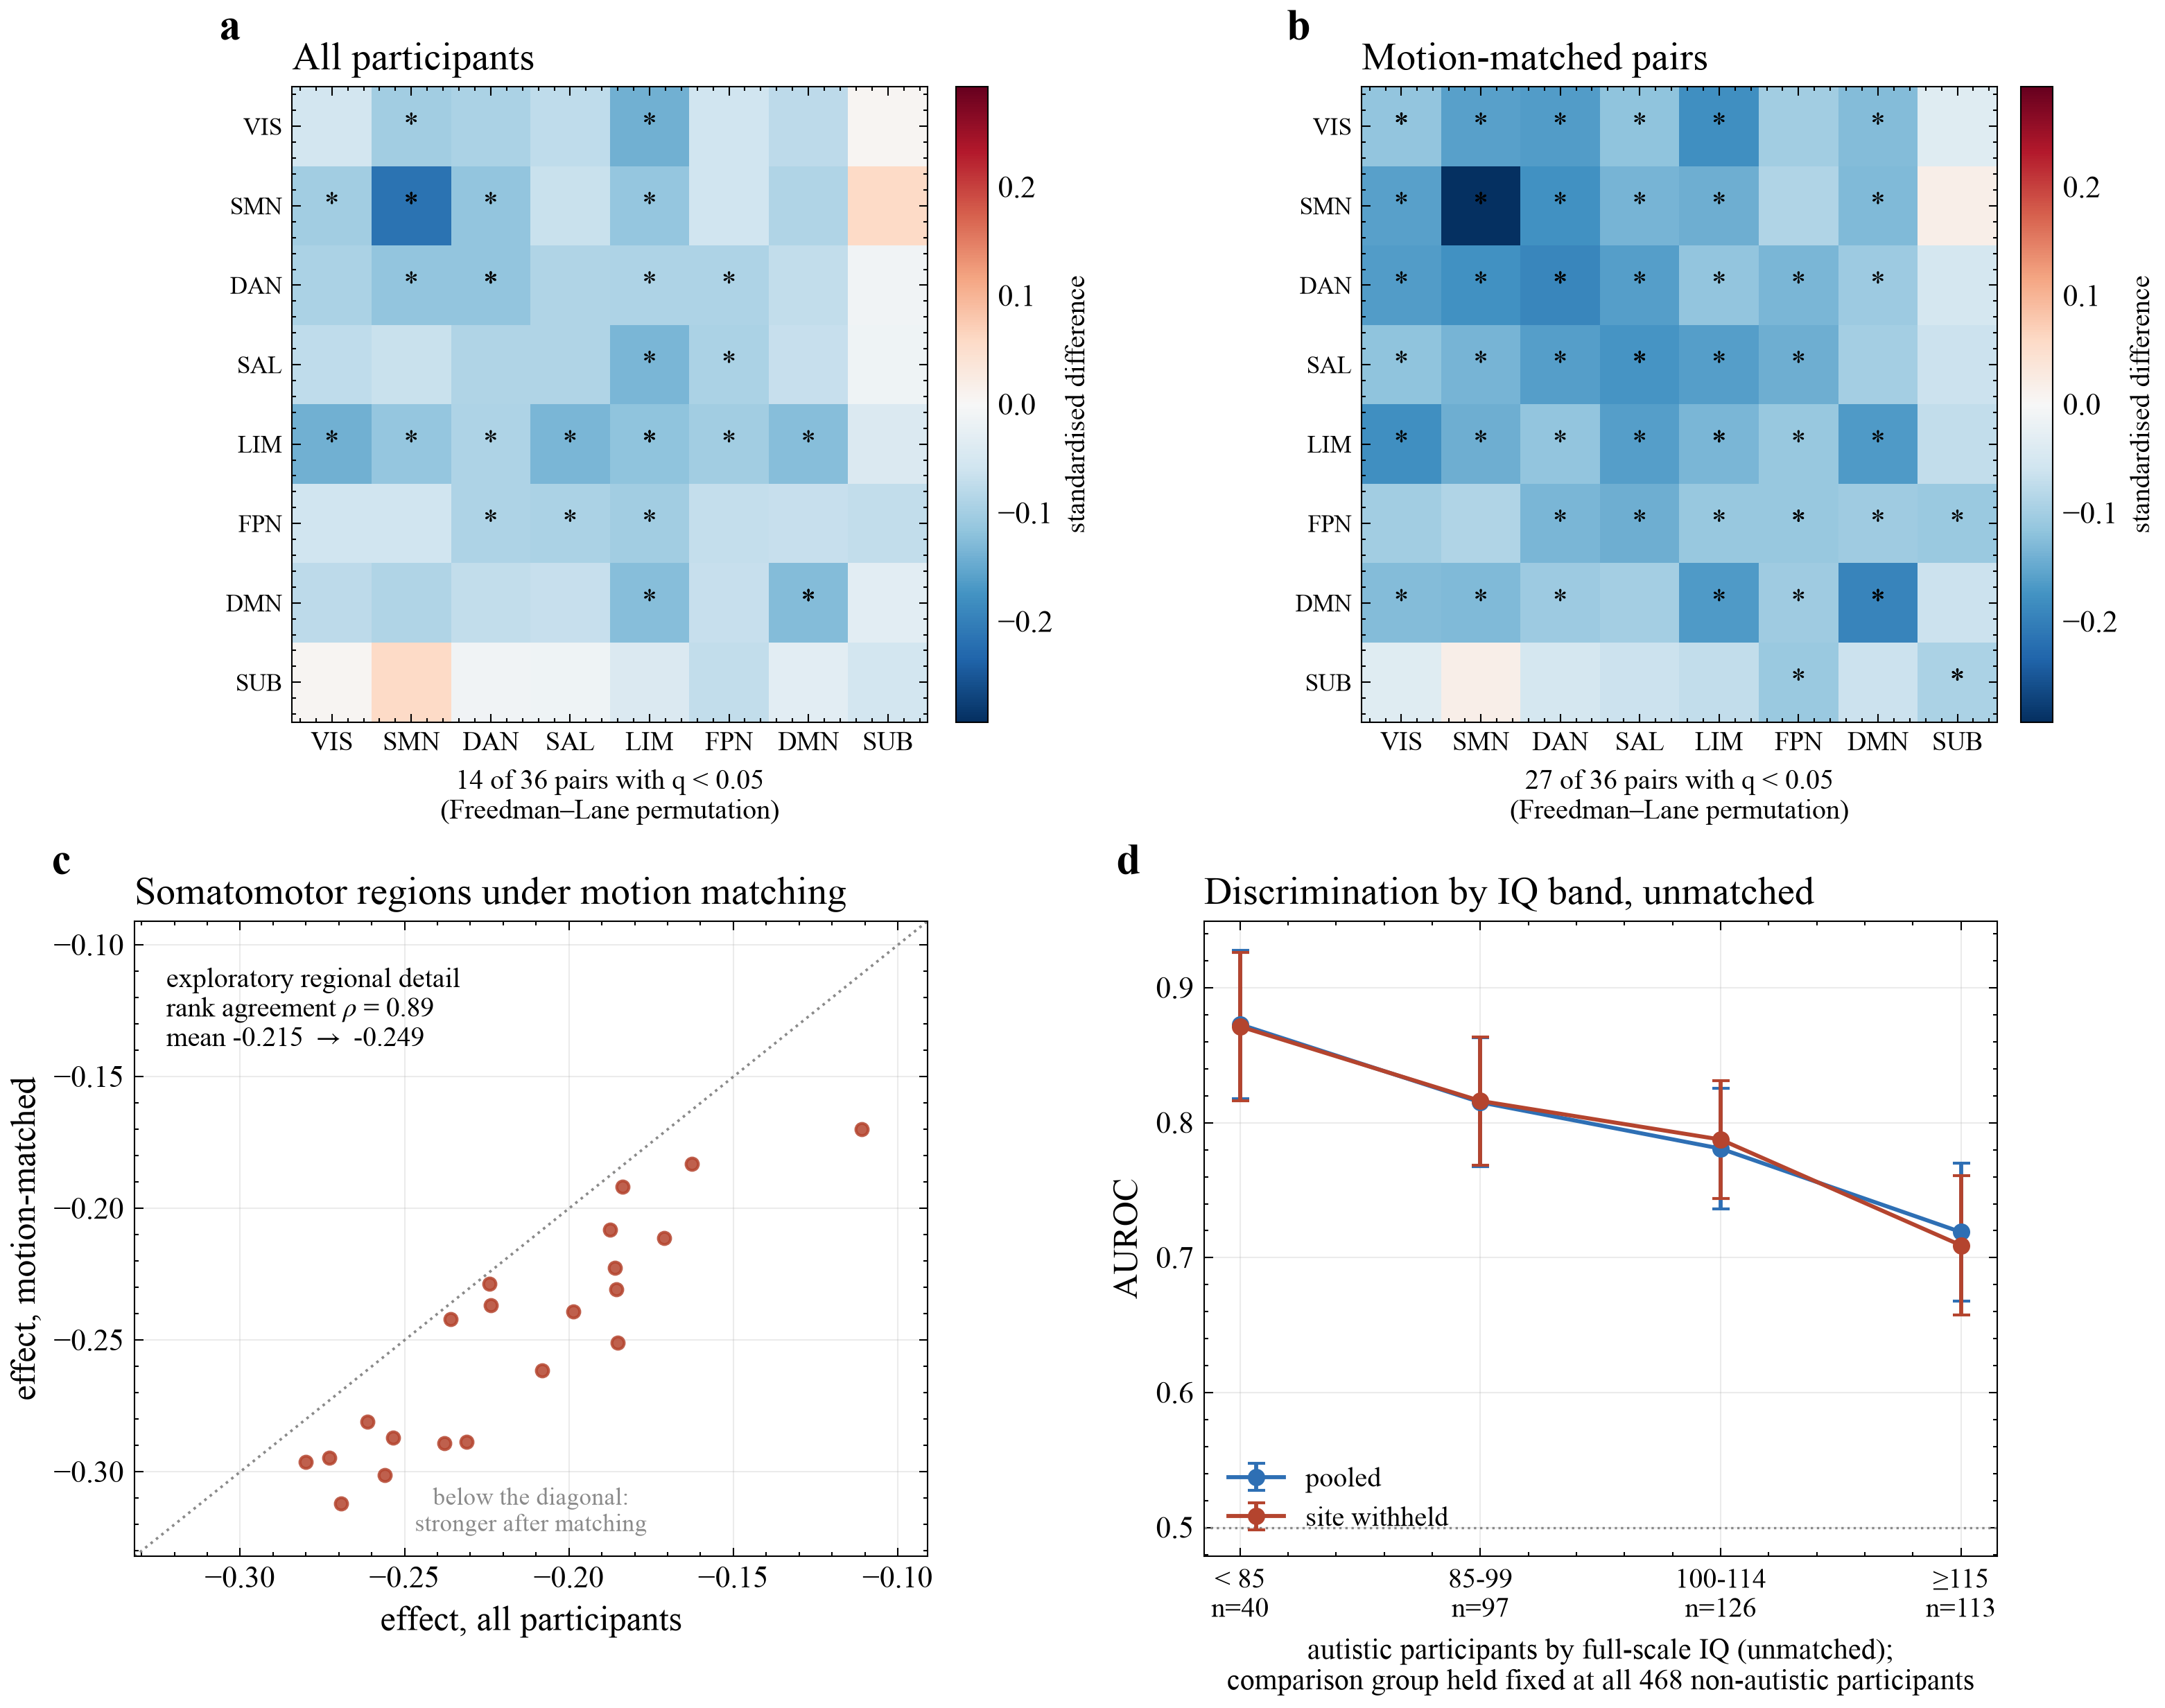
\includegraphics[width=\linewidth]{fig_groupdiff}
\caption{Group differences in functional-system connectivity and the effect of motion
matching. (a, b) Standardised difference for every pair of systems (system codes as in Figure~\ref{fig:overview}) in all participants and
in within-site pairs matched for head motion, on a shared colour scale; asterisks mark pairs with BH-FDR $q<0.05$ under Freedman--Lane permutation, and colours show the standardised differences. (c) The effect of each somatomotor region in all participants plotted against its effect in motion-matched pairs (exploratory); points below the diagonal are stronger once motion is matched. (d) Discrimination by full-scale IQ band among
autistic participants (below 85, 85--99, 100--114, and 115 or above), each against all 468 non-autistic participants, under both validation protocols; the bands are not matched on IQ to the comparison group.}
\label{fig:group-differences}
\end{figure}

The same pattern is observed when both groups are divided into quartiles of site-centred full-scale IQ (Table~\ref{tab:iq-quartiles}). Under pooled ten-fold validation, AUROC decreases from 0.833 in the lowest quartile to 0.709 in the highest. Because autistic participants have lower full-scale IQ overall (Table~\ref{tab:participants}), this stratified comparison may still reflect differences in IQ between the groups. To reduce this imbalance, autistic participants are matched to non-autistic participants from the same site within five full-scale IQ points. This produces 274 matched pairs under pooled ten-fold validation and 275 pairs under LOSO validation.

\begin{table}[t]
\centering
\caption{AUROC by quartile of site-centred full-scale IQ, in all participants and in
participants matched on full-scale IQ within site. The matched counts are given for pooled
ten-fold and LOSO validation, respectively.}
\label{tab:iq-quartiles}
\small
\begin{tabular}{@{}lcccccc@{}}
\toprule
 & \multicolumn{3}{c}{All participants} & \multicolumn{3}{c}{IQ-matched participants} \\
\cmidrule(lr){2-4}\cmidrule(l){5-7}
Quartile & $n$ & Pooled ten-fold & LOSO & $n$ (pooled / LOSO) & Pooled ten-fold & LOSO \\
\midrule
Q1 & 204 & 0.833 & 0.825 & 137 / 144 & 0.855 & 0.848 \\
Q2 & 203 & 0.794 & 0.793 & 137 / 132 & 0.700 & 0.735 \\
Q3 & 201 & 0.746 & 0.745 & 138 / 137 & 0.751 & 0.737 \\
Q4 & 203 & 0.709 & 0.705 & 136 / 137 & 0.756 & 0.756 \\
\bottomrule
\end{tabular}
\end{table}

After IQ matching, discrimination remains highest in the lowest quartile but no longer declines consistently across the upper three. Under pooled ten-fold validation, AUROC is 0.855 in the lowest quartile and ranges from 0.700 to 0.756 in the remaining quartiles; under LOSO validation, the corresponding values are 0.848 and 0.735--0.756. This suggests that part of the original IQ gradient reflects between-group differences in IQ. Complementary within-group analyses show a negative association between classifier score and cognitive ability among autistic participants, but not among non-autistic participants. After adjustment for site, age, and mean FD, the pooled ten-fold score correlates with full-scale IQ at $\rho=-0.180$ ($p=0.0004$, $n=376$) in autistic participants, compared with $\rho=+0.048$ ($p=0.3208$, $n=435$) in non-autistic participants. Similar patterns are observed for verbal and performance IQ and under both validation protocols. Diagnosis-by-IQ interaction models further test this difference directly while adjusting for age, sex, mean FD, and site. The interaction remains significant after BH-FDR correction for full-scale IQ ($\beta=-0.176$, $q=0.025$) and verbal IQ ($\beta=-0.205$, $q=0.025$) under pooled ten-fold validation, and for both measures under LOSO validation ($q=0.033$). The interaction for performance IQ does not survive correction ($q=0.082$). These results indicate that the negative association between classifier score and cognitive ability is stronger in autistic participants for full-scale and verbal IQ.

\begin{table}[t]
\centering
\caption{Spearman correlation between classifier score and IQ within each diagnostic group, reported as $\rho$ ($p$). Before correlation, both variables are residualised for site, age, and mean FD. The p-values are not adjusted for multiple comparisons.}
\label{tab:iq-correlations}
\small
\setlength{\tabcolsep}{4pt}
\begin{tabular}{@{}lccccc@{}}
\toprule
 & & \multicolumn{2}{c}{Autistic} & \multicolumn{2}{c}{Non-autistic} \\
\cmidrule(lr){3-4}\cmidrule(l){5-6}
Measure & $n$ (autistic / non-autistic) & Pooled ten-fold & LOSO & Pooled ten-fold & LOSO \\
\midrule
Full-scale IQ & 376 / 435 & $-0.180$ (0.0004) & $-0.179$ (0.0005) & $+0.048$ (0.3208) & $+0.022$ (0.6466) \\
Verbal IQ & 342 / 379 & $-0.182$ (0.0007) & $-0.189$ (0.0004) & $+0.039$ (0.4547) & $+0.001$ (0.9892) \\
Performance IQ & 344 / 391 & $-0.152$ (0.0047) & $-0.147$ (0.0062) & $+0.007$ (0.8862) & $-0.005$ (0.9271) \\
\bottomrule
\end{tabular}
\end{table}

The absence of a comparable score--IQ association in non-autistic participants argues against a general relation between cognitive ability and classifier score (Table~\ref{tab:iq-correlations}). This interpretation is strengthened by the diagnosis-by-IQ interaction results, which remain significant for full-scale and verbal IQ, although full-scale IQ varies less among non-autistic participants (Table~\ref{tab:participants}). The association is also consistent with the verbal-IQ dependence reported in ABIDE by \citet{Nielsenetal2013}. However, the IQ-matched upper quartiles do not show a monotonic decline in AUROC, so the exploratory analyses do not establish a simple IQ-specific gradient in detectability. Instead, they indicate that measured ABIDE-I performance varies with the cognitive composition of the autistic sample, such that the same method can yield different AUROC values in cohorts with different IQ distributions. No corresponding reduction in discrimination is observed among female participants. Under pooled ten-fold validation, AUROC is 0.827 (0.760--0.895, $n=144$) in female participants and 0.764 (0.730--0.798, $n=727$) in male participants; under LOSO validation, the corresponding values are 0.806 (0.735--0.878) and 0.767 (0.733--0.801). Because these intervals overlap and the female subgroup is small, no sex difference in discrimination is inferred.

\subsection{Functional-system differences under motion matching}
\label{subsec:results-system-differences}

Functional-system differences are examined as exploratory group contrasts, and the motion-matched somatomotor result contributes to the third study contribution. To reduce the 19,110 connection-level effects to a more interpretable scale, regions are grouped into the seven cortical systems of \citet{Yeoetal2011} plus a subcortical/cerebellar class, producing 36 system pairs with 21--1,462 connections each (median 441). Connection values are adjusted for acquisition site, mean framewise displacement, age, and sex. Because diagnosis is associated with age, sex, and mean FD, inference uses Freedman--Lane residual permutation within site, which preserves this association in every permutation, and the within-site permutation of residualised connections is reported as a sensitivity analysis. In the 863-participant group-contrast cohort, 14 of 36 system pairs differ after BH-FDR correction under Freedman--Lane permutation, all with lower connectivity in autistic participants (Table~\ref{tab:system-pairs}; Figure~\ref{fig:group-differences}a). The 10 pairs identified by the sensitivity analysis are all among them, and the Freedman--Lane effects and the standardised differences rank the 36 pairs identically (Spearman $\rho=1.0$). Four of the 14 pairs have $q=0.0499$, just below the threshold, so the 10 pairs identified by both procedures form the more robust set. Overall, 34 of 36 system-pair effects are negative, with no significant increases. The largest reduction occurs within the somatomotor system (Freedman--Lane effect $-0.226$, $q=0.002$; standardised difference $-0.215$), while the limbic system shows differences across the widest range of system pairs. Because both nuisance adjustment and permutation account for site, these effects reflect group differences after controlling for site-related variation in connectivity.

\begin{table}[t]
\centering
\caption{Functional-system pairs with lower connectivity in autistic participants under Freedman--Lane residual permutation in the 863-participant group-contrast cohort. Effects are adjusted for site, age, sex, and mean FD. Fourteen of 36 pairs survive BH-FDR correction ($q<0.05$), with none showing higher connectivity. Standardised differences and within-site permutation $q$-values are shown for comparison.}
\label{tab:system-pairs}
\footnotesize
\setlength{\tabcolsep}{3pt}
\begin{tabular}{@{}llcccccc@{}}
\toprule
 & & & \multicolumn{2}{c}{Freedman--Lane} & \multicolumn{2}{c}{Within-site permutation} \\
\cmidrule(lr){4-5}\cmidrule(l){6-7}
System & System & Connections & Effect & $q$ & Std. difference & $q$ \\
\midrule
Somatomotor & Somatomotor & 210 & $-$0.226 & 0.0024 & $-$0.215 & 0.0024 \\
Limbic & Visual & 210 & $-$0.147 & 0.0024 & $-$0.140 & 0.0024 \\
Limbic & Salience / ventral attention & 147 & $-$0.140 & 0.0072 & $-$0.133 & 0.0130 \\
Default mode & Default mode & 903 & $-$0.133 & 0.0024 & $-$0.127 & 0.0024 \\
Default mode & Limbic & 301 & $-$0.131 & 0.0036 & $-$0.125 & 0.0036 \\
Limbic & Limbic & 21 & $-$0.124 & 0.0144 & $-$0.118 & 0.0144 \\
Dorsal attention & Somatomotor & 399 & $-$0.122 & 0.0274 & $-$0.116 & 0.0245 \\
Dorsal attention & Dorsal attention & 171 & $-$0.121 & 0.0152 & $-$0.115 & 0.0237 \\
Limbic & Somatomotor & 147 & $-$0.119 & 0.0152 & $-$0.114 & 0.0245 \\
Frontoparietal control & Limbic & 147 & $-$0.107 & 0.0152 & $-$0.102 & 0.0245 \\
Somatomotor & Visual & 630 & $-$0.106 & 0.0499 & $-$0.101 & 0.0576 \\
Frontoparietal control & Salience / ventral attention & 441 & $-$0.097 & 0.0499 & $-$0.093 & 0.0576 \\
Dorsal attention & Frontoparietal control & 399 & $-$0.096 & 0.0499 & $-$0.091 & 0.0576 \\
Dorsal attention & Limbic & 133 & $-$0.095 & 0.0499 & $-$0.091 & 0.0576 \\
\bottomrule
\end{tabular}
\end{table}

Because both procedures operate on residualised connections, a separate motion-matched analysis is used to examine whether the group differences persist when autistic and non-autistic participants are closely matched on mean FD within site (Section~\ref{subsubsec:system-motion-regional}). Under the system-level caliper, 256 pairs are retained and the group difference in motion is removed ($p=7.6\times10^{-7}$ before matching and $p=0.59$ after). In this matched sample, 27 of 36 system pairs are significant under Freedman--Lane permutation (26 under the sensitivity analysis), compared with 14 of 36 (10) in the full cohort, although the change in count cannot be attributed to motion matching alone because the matched sample also differs in size and composition. The somatomotor within-system Freedman--Lane effect strengthens from $-0.226$ to $-0.294$, and the standardised difference from $-0.2155$ ($z=-4.77$) to $-0.2925$ ($z=-4.89$). The regional analysis within the somatomotor system is exploratory, because the system is chosen after inspection of the system-level results and the BH-FDR correction across its 21 regions does not account for that choice. Descriptively, all 21 regional effects are negative in the full cohort, with the strongest in the postcentral gyrus, paracentral lobule, and precentral gyrus. Using the wider regional caliper, 280 matched pairs are retained and the motion difference is again removed ($p=0.28$). Every regional effect is more negative in the matched sample than in the full cohort, and the ordering is preserved (rank correlation 0.89), while the mean regional effect changes from $-0.215$ to $-0.249$ (Figure~\ref{fig:group-differences}c); the matched and full samples differ in size and composition, and neighbouring regional effects are correlated, so this pattern is descriptive. Under Freedman--Lane permutation the 21 regions also remain below $q=0.05$ in the full and matched analyses, with a mean regional effect of $-0.226$ and $-0.294$ on the regression scale, which is not directly comparable with the standardised regional effects above. The regional ranking shows moderate internal stability, with a split-half correlation of 0.55 across the 21 regions, compared with 0.38 for all 210 within-system connections and 0.34 for the top 50. Random blocks of 21 regions have a median stability of 0.35, and 9\% reach the somatomotor value. Mean FD is positively associated with mean connection strength ($\rho=+0.51$ across participants and $+0.45$ within site), and the same holds within the somatomotor system: after removing site, mean FD correlates positively with all 210 within-somatomotor connections (mean $\rho=0.18$), and the shift in these connections that the group difference in mean FD would produce through this linear relation is $+0.006$ in Fisher-transformed correlation, whereas the observed site-adjusted group difference is $-0.046$. The somatomotor reduction is therefore not readily explained by the recorded relation between mean FD and connectivity, although this check is linear and cannot exclude other motion effects. The somatomotor finding is consistent with earlier reports \citep{Chenetal2015,Holigaetal2019,Ilioskaetal2023}, although overlap in ABIDE participants prevents treating this agreement as independent replication. Overall, the somatomotor reduction persists and strengthens after matching on recorded mean FD, but residual motion cannot be fully excluded, the contrasts do not show which features the classifier uses, and the results remain conditional on the chosen preprocessing strategy without global signal regression.

\subsection{Feature-selection scope and granularity}
\label{subsec:results-selection-scope}

The effect of data-access scope on measured performance is examined across seven conditions using identical folds and the 19,900 static tangent features of the primary cohort (Section~\ref{par:selection-scope}; Table~\ref{tab:selection-scope}). These analyses are reported as methodological checks rather than as study contributions. Fitting the tangent reference globally, or fitting both the reference and scaler globally, changes fold-mean AUROC by no more than 0.003. Similarly, selecting the regularisation constant on the held-out fold gives an AUROC of 0.758, while adding acquisition site as a predictor gives 0.756. These results show that these changes in data-access scope have little effect on performance compared with the much larger effect of label-informed feature selection examined next.

\begin{table}[t]
\centering
\caption{Fold-mean AUROC across seven data-access conditions, evaluated using 19,900 static tangent features in the primary cohort of 871 participants with identical outer folds. SD is calculated across the outer folds.}
\label{tab:selection-scope}
\small
\begin{tabular}{@{}>{\raggedright\arraybackslash}p{0.62\linewidth}cc@{}}
\toprule
Condition & AUROC & SD \\
\midrule
Reference: every step fitted within the training partition & 0.756 & 0.048 \\
Tangent reference fitted on all participants & 0.756 & 0.048 \\
Tangent reference and scaler fitted on all participants & 0.753 & 0.049 \\
Regularisation constant chosen on the held-out fold & 0.758 & 0.048 \\
Acquisition site added as a predictor & 0.756 & 0.049 \\
Tangent reference fitted on all participants and 2,000 of 19,900 connections selected with all diagnostic labels & 0.987 & 0.008 \\
All five changes combined & 0.988 & 0.008 \\
\bottomrule
\end{tabular}
\end{table}

In contrast, selecting 2,000 of 19,900 connections with an F test using all diagnostic labels before CV raises fold-mean AUROC from 0.756 to 0.987 and accuracy from 0.692 to 0.948 on the same folds. Because fitting the tangent reference globally leaves AUROC unchanged at 0.756, the increase is driven primarily by the label-informed selection step. Applying all data-access changes together gives an AUROC of 0.988, showing little additional effect beyond selection. Thus, among the tested conditions, only global connection-level feature selection changes AUROC by more than 0.003, whereas held-out tuning and the other scope changes have minimal effects. Estimates from pipelines that select connections before CV are therefore not directly comparable with estimates from nested selection. Region-level selection shows a different pattern (Table~\ref{tab:region-selection}; Figure~\ref{fig:corrections}c). Ranking regions with all labels or with training-fold labels changes AUROC by only 0.006 on average across models retaining 10--100 of 196 regions, with differences ranging from 0.001 at 10 regions to 0.012 at 100 and no consistent direction. Refitting the nuisance model within each outer-training partition changes the training-fold condition by only 0.0035 on average and at most 0.0085, while preserving the ordering across list lengths; all restricted models remain below the model using all 196 regions (0.781). These findings are consistent with greater sensitivity of fine-grained connection selection to label access than region-level selection. However, the two analyses also differ in cohort size, shrinkage, ranking statistic, and AUROC summary, so feature granularity cannot be isolated as the only explanation.

\begin{table}[t]
\centering
\caption{Participant-pooled AUROC when the top-ranked regions are chosen with all
diagnostic labels or with the labels of each training fold only, in the group-contrast
cohort (863 participants and 196 regions). All 196 regions give 0.781.}
\label{tab:region-selection}
\small
\begin{tabular}{@{}ccc@{}}
\toprule
Regions kept & Chosen with all labels & Chosen within each fold \\
\midrule
10 & 0.628 & 0.627 \\
20 & 0.660 & 0.656 \\
30 & 0.699 & 0.702 \\
50 & 0.738 & 0.748 \\
100 & 0.764 & 0.752 \\
\bottomrule
\end{tabular}
\end{table}

\begin{figure}[pos=tbp]
\centering
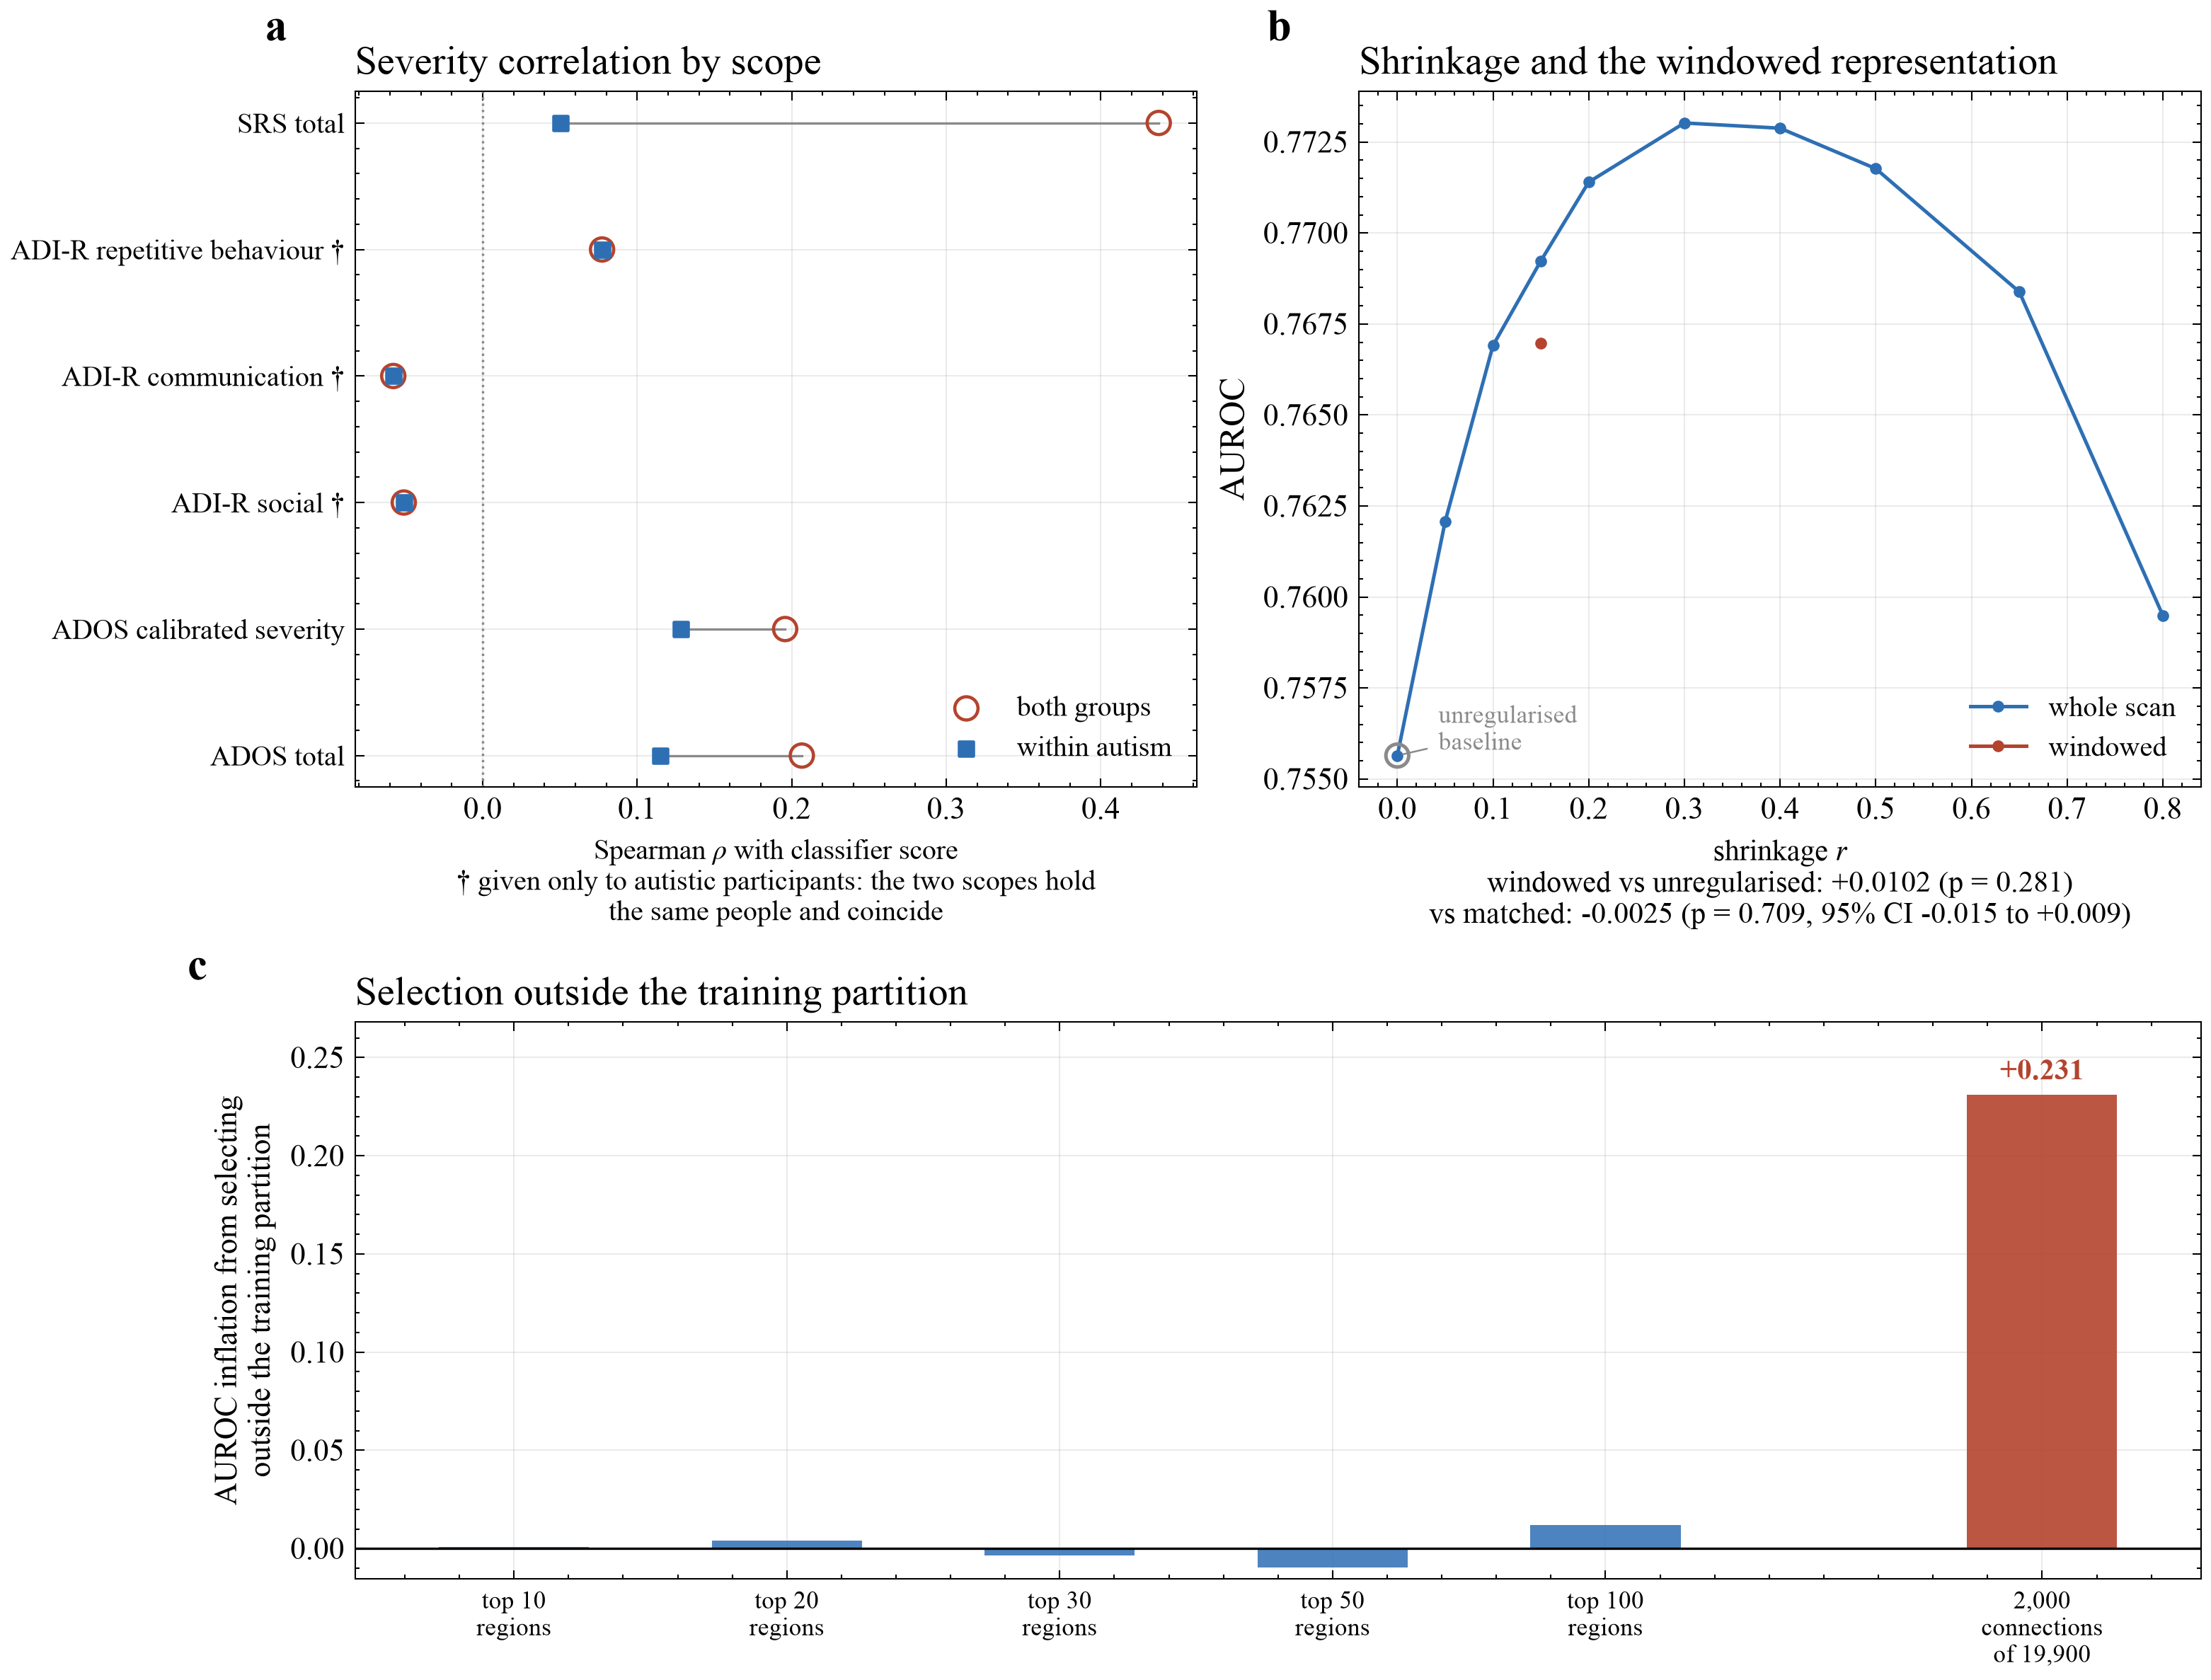
\includegraphics[width=\linewidth]{fig_corrections}
\caption{Three effects that change when the corresponding control is applied. (a)
Correlation between classifier score and symptom severity under pooled ten-fold validation,
computed across both groups and within the autistic group; rows marked with a dagger are
instruments given only to autistic participants, for which the two scopes necessarily coincide.
(b) AUROC of whole-scan connectivity across shrinkage levels, with the windowed
representation placed at the shrinkage that it applies to its own windows. (c) AUROC
inflation from selection outside the training partition, for 10 to 100 of 196 regions and
for 2,000 of 19,900 connections.}
\label{fig:corrections}
\end{figure}

Restricting the model to the most discriminating regions reduces performance at every list length. Using all 196 regions gives an AUROC of 0.781, higher than any reduced set in Table~\ref{tab:region-selection}, while the smallest subset is lower by 0.154. This pattern suggests that discriminative information is distributed across many regions rather than concentrated only in those with the largest group differences. Region restriction therefore provides no performance advantage in these data. More broadly, the published accuracy range is already reached without feature selection before the split. In the wider cohort, the ensemble achieves a participant-pooled accuracy of 0.706 under pooled ten-fold validation (Section~\ref{subsec:results-performance}), compared with published values of 0.700, 0.703, and 0.708 for the same eligible count of 1,035 participants. Accuracy at this level therefore does not require selection outside the training partition.

\subsection{Classifier configurations}
\label{subsec:results-classifier-family}

Linear classifiers perform better than the evaluated fixed-configuration tree ensembles on static tangent connectivity, forming part of the fifth study contribution. All eight classifiers use the same features, scaling procedure, and outer folds (Section~\ref{par:classifier-family}), so the comparison is made under a common input and validation setting. The five linear classifiers achieve participant-pooled AUROCs of 0.735--0.757, compared with 0.611--0.624 for random forest, XGBoost, and CatBoost (Table~\ref{tab:classifier-family}). Penalised logistic regression gives the highest AUROC at 0.757, followed closely by ridge classification at 0.755 and linear SVC at 0.753. Shrinkage LDA and the rank-20 spectral model achieve AUROCs of 0.741 and 0.735, respectively. Because only logistic regression is tuned, these results compare the specified classifier configurations rather than the best attainable performance of each model family.

\begin{table}[t]
\centering
\caption{Classifier configurations on the static tangent features of the primary cohort
(871 participants), with identical features, scaling and outer folds. Only logistic
regression is tuned; the other classifiers use fixed configurations.}
\label{tab:classifier-family}
\small
\setlength{\tabcolsep}{4pt}
\begin{tabular}{@{}lcccc@{}}
\toprule
Classifier & AUROC (participant-pooled) & AUROC (fold mean) & SD (folds) & Accuracy (fold mean) \\
\midrule
Logistic regression & 0.757 & 0.756 & 0.048 & 0.692 \\
Ridge & 0.755 & 0.755 & 0.047 & 0.693 \\
Linear SVC & 0.753 & 0.753 & 0.048 & 0.687 \\
Shrinkage LDA (PCA-200) & 0.741 & 0.739 & 0.052 & 0.669 \\
Low-rank spectral (rank 20) & 0.735 & 0.737 & 0.044 & 0.672 \\
CatBoost & 0.624 & 0.623 & 0.042 & 0.597 \\
XGBoost & 0.617 & 0.616 & 0.050 & 0.584 \\
Random forest & 0.611 & 0.609 & 0.049 & 0.577 \\
\bottomrule
\end{tabular}
\end{table}

The performance gap between logistic regression and the tree ensembles is substantial. Logistic regression exceeds XGBoost by 0.1396 AUROC, random forest by 0.1461, and CatBoost by 0.1327, with unadjusted DeLong $p$-values ranging from $6.3\times10^{-15}$ to $2.4\times10^{-12}$ (Section~\ref{subsubsec:paired-comparisons}). By comparison, the rank-20 spectral model is 0.0214 below logistic regression (unadjusted $p=0.0439$; $q=0.1065$, reported for reference only). These results describe the specific configurations evaluated rather than the best possible performance of each classifier family, because only logistic regression is tuned while the tree ensembles use fixed settings (Section~\ref{par:classifier-family}). However, the fixed-configuration ridge, linear SVC, and LDA models also outperform all three tree ensembles. The stronger performance of the linear configurations therefore cannot be explained by logistic-regression tuning alone.

\subsection{Scope of the symptom-severity associations}
\label{subsec:results-symptom-severity}

The symptom analyses show that classifier scores are associated with symptom measures mainly when both diagnostic groups are analysed together, forming part of the fourth study contribution (Figure~\ref{fig:corrections}a). Under pooled ten-fold validation, 3 of 6 associations survive BH-FDR correction across both groups, whereas none survives within autistic participants alone (Section~\ref{par:symptom-associations}). The clearest example is the SRS total, for which the correlation falls from $\rho=0.438$ across both groups ($n=300$) to 0.050 within autistic participants ($n=163$). The corresponding values are 0.207 versus 0.115 for ADOS total and 0.196 versus 0.128 for ADOS calibrated severity. For the ADI-R domains, the correlations are unchanged because these measures are available only for autistic participants. These results indicate that the pooled associations largely reflect diagnostic-group separation, while an association between classifier score and symptom severity within autistic participants is not established.

\subsection{Windowed connectivity and covariance shrinkage}
\label{subsec:results-windowed-shrinkage}

The apparent advantage of windowed connectivity is small and is not retained when the whole-scan representation receives the same additional covariance shrinkage, forming part of the fifth study contribution (Figure~\ref{fig:corrections}b). The windowed representation applies an additional shrinkage of 0.15 to its covariance estimates, whereas the original static representation does not (Section~\ref{subsubsec:primary-comparisons}). Applying the same shrinkage to the static representation increases its AUROC by 0.013 (unadjusted DeLong $p=0.004$). By comparison, the windowed representation exceeds the unshrunk static baseline by 0.010 ($p=0.281$) but differs from the shrinkage-matched static baseline by only $-0.002$ ($p=0.709$). Thus, no additional benefit of windowing is detected beyond matched shrinkage. The difference from the shrinkage-matched static baseline is $-0.002$ (95\% site-clustered bootstrap interval $-0.015$ to $+0.009$), which excludes a windowed advantage larger than about 0.009 AUROC but not a smaller one.

\subsection{Calibration and recalibration within the training partitions}
\label{subsec:results-calibration}

The native ensemble probabilities show calibration slopes close to one but a small systematic offset in their average predicted risk, and training-partition recalibration removes this offset without changing discrimination; this forms the first study contribution (Table~\ref{tab:calibration-recalibration}; Figure~\ref{fig:calibration}). Under pooled ten-fold validation, the native calibration slope is 1.117 (95\% site-clustered bootstrap interval 0.901--1.325), and under LOSO validation it is 1.120 (0.866--1.366), with both intervals including one. Calibration-in-the-large is $-0.162$ ($-0.287$ to $-0.048$) under pooled validation and $-0.181$ ($-0.389$ to 0.019) under LOSO validation, indicating that the native probabilities tend to overestimate autism prevalence on average. The Brier score is 0.194 under both protocols, corresponding to Brier skill scores of 0.221 and 0.218 relative to a prevalence-only model. ECE varies with the binning choice: under pooled validation it is 0.037 with five bins, 0.046 with ten, and 0.059 with twenty, while the smallest bins contain 86, 17, and 0 participants, respectively. ECE is therefore reported together with the number of bins rather than as a single standalone calibration measure (Figure~\ref{fig:calibration}a,b).

\begin{table}[t]
\centering
\caption{Ensemble probabilities are evaluated before and after recalibration fitted within each outer training partition. Calibration-in-the-large, where negative values indicate over-prediction of autism, and the calibration slope are reported with 95\% site-clustered bootstrap intervals. ECE is calculated using ten equal-width bins, and accuracy is measured at a threshold of 0.5. The final row of each block is included as a diagnostic, with the ensemble members refitted using an unpenalised intercept.}
\label{tab:calibration-recalibration}
\footnotesize
\setlength{\tabcolsep}{3pt}
\begin{tabular}{@{}lcccccc@{}}
\toprule
Correction & Calibration-in-the-large & Slope & Brier & ECE & AUROC & Accuracy \\
\midrule
\multicolumn{7}{@{}l}{\textit{Pooled ten-fold validation}} \\
Native & $-0.162$ ($-0.287$ to $-0.048$) & 1.117 (0.901 to 1.325) & 0.194 & 0.046 & 0.776 & 0.707 \\
Intercept (primary) & $-0.010$ ($-0.136$ to 0.103) & 1.115 (0.898 to 1.324) & 0.193 & 0.040 & 0.776 & 0.713 \\
Logistic & $-0.010$ ($-0.143$ to 0.105) & 1.026 (0.824 to 1.218) & 0.192 & 0.037 & 0.776 & 0.711 \\
Isotonic & 0.000 ($-0.139$ to 0.117) & 0.855 (0.654 to 1.043) & 0.194 & 0.018 & 0.771 & 0.707 \\
Unpenalised intercept (diagnostic) & $+0.061$ ($-0.066$ to 0.175) & 1.114 (0.902 to 1.316) & 0.193 & 0.044 & 0.776 & 0.720 \\
\midrule
\multicolumn{7}{@{}l}{\textit{LOSO validation}} \\
Native & $-0.181$ ($-0.389$ to 0.019) & 1.120 (0.866 to 1.366) & 0.194 & 0.040 & 0.774 & 0.711 \\
Intercept (primary) & $+0.023$ ($-0.186$ to 0.235) & 1.115 (0.860 to 1.366) & 0.194 & 0.027 & 0.774 & 0.701 \\
Logistic & $+0.012$ ($-0.189$ to 0.227) & 1.159 (0.899 to 1.493) & 0.195 & 0.033 & 0.769 & 0.705 \\
Isotonic & $-0.006$ ($-0.214$ to 0.228) & 0.989 (0.733 to 1.284) & 0.197 & 0.021 & 0.766 & 0.698 \\
Unpenalised intercept (diagnostic) & $+0.036$ ($-0.180$ to 0.256) & 1.105 (0.857 to 1.353) & 0.194 & 0.030 & 0.772 & 0.705 \\
\bottomrule
\end{tabular}
\end{table}



\begin{figure}[pos=tbp]
\centering
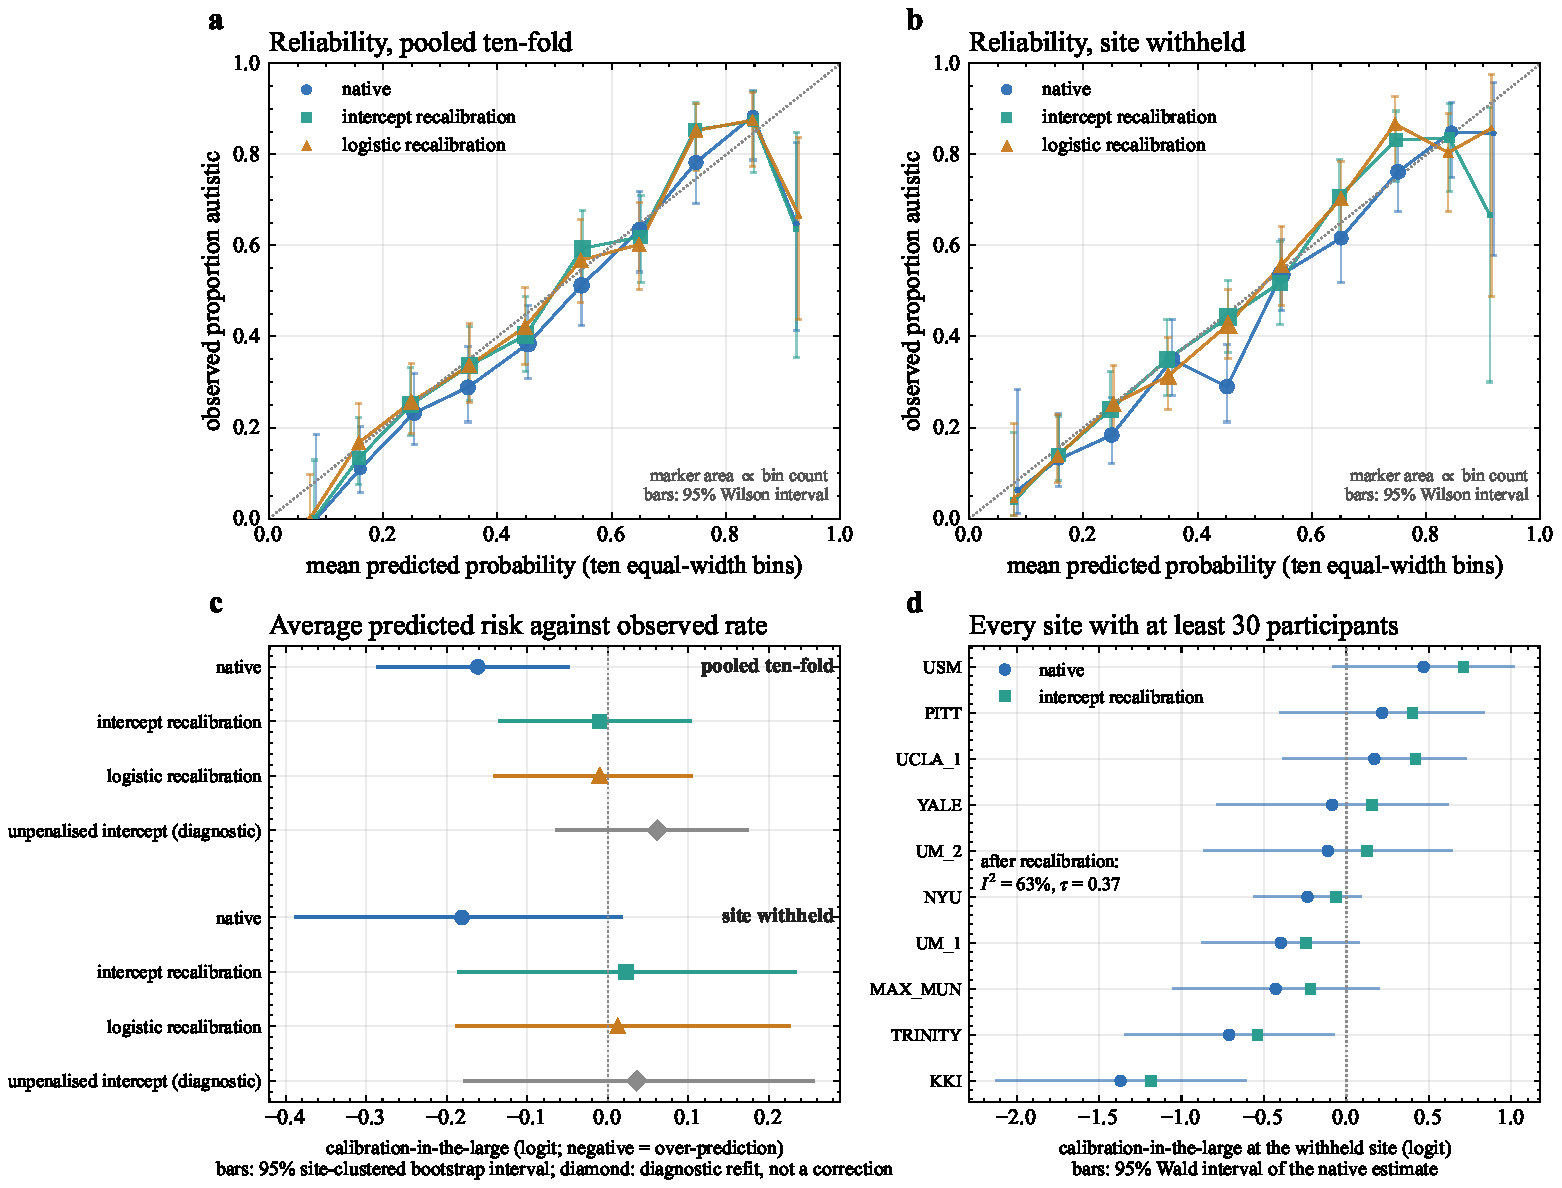
\includegraphics[width=\linewidth]{fig_calibration}
\caption{Calibration of the ensemble probabilities under pooled ten-fold and LOSO validation. Reliability curves compare native and training-only recalibrated probabilities. Calibration-in-the-large is shown with 95\% site-clustered bootstrap intervals, including the unpenalised-intercept diagnostic, while site-level offsets are reported for withheld sites with at least 30 participants.}
\label{fig:calibration}
\end{figure}


The calibration offset is consistent with intercept penalisation in the original solver. Because the intercept is penalised together with the feature weights, it is drawn towards zero and shifts predicted probabilities towards 0.5. The mean fitted intercept is $-0.017$; refitting with an unpenalised intercept moves it to $-0.253$ and shifts calibration-in-the-large from $-0.162$ to $+0.061$ under pooled validation and from $-0.181$ to $+0.036$ under LOSO validation. Because the corrected values slightly cross zero, this diagnostic supports intercept penalisation as an important contributor rather than the sole cause of miscalibration. The primary intercept-only recalibration, fitted within each outer training partition, reduces calibration-in-the-large to $-0.010$ under pooled validation and $+0.023$ under LOSO validation, while AUROC remains essentially unchanged. More flexible logistic and isotonic recalibration provide no consistent additional benefit. At the fixed threshold of 0.5, recalibration lowers sensitivity and increases specificity, with little change in overall accuracy, showing that calibration affects the operating point even when discrimination is preserved. Site-level calibration is less uniform. After recalibration, heterogeneity is negligible under pooled validation ($I^2=0\%$) but remains substantial under LOSO validation ($I^2=63\%$). The remaining site offsets are consistent with differences in autistic prevalence across sites. Overall, intercept-only recalibration corrects the average probability offset without reducing discrimination, although site-specific calibration differences remain.

\subsection{Attribution of the score to functional-system pairs}
\label{subsec:results-interpretation}

The score of each linear ensemble member is attributed exactly to the \reviewdel{36 functional-system pairs}\reviewhl{36 functional-system pairs plus one unassigned connection group}, and the average of the three member scores, which closely approximates the adopted probability-mean ensemble, is attributed in the same way; this attribution forms the second contribution of the study (Table~\ref{tab:system-contributions}; Figure~\ref{fig:interpretation}). Reproducibility is observed at the system-pair level, with weaker reproducibility found for individual connections. Each held-out member score is reproduced by the summed pair contributions within $10^{-14}$, and the stored probabilities are reproduced by the stored weights within $10^{-7}$. The average of the three member scores has a participant-pooled AUROC of 0.7759, compared with 0.7760 for the probability-mean ensemble, correlates with it at Spearman $\rho=0.999$, and classifies 0.2\% of participants differently at the 0.5 threshold (LOSO: 0.7746 against 0.7745, $\rho=0.999$, 0.1\%). Averaged across the three views, between-group separation of the member scores is 1.07 logit units under pooled validation and 1.06 when a site is withheld, compared with 1.00 and 0.98 for the logit of the probability-mean ensemble, so the shares reported below describe the averaged member scores and slightly overstate the separation of the ensemble probability. Zero is excluded from the contribution-difference intervals for 28 of the 37 connection groups under pooled validation and for 28 groups under site-held-out validation, with no negative contribution difference observed (Figure~\ref{fig:interpretation}a). The separation is therefore distributed across many functional-system pairs rather than being concentrated in a small number of pairs.

\begin{table}[t]
\centering
\caption{Functional-system pairs contributing most to held-out group separation across the three ensemble views. Shares are reported with 95\% site-clustered bootstrap intervals, and pairwise AUROCs are tested against a familywise permutation reference across all 36 pairs.}
\label{tab:system-contributions}
\footnotesize
\setlength{\tabcolsep}{3pt}
\begin{tabular}{@{}llcccc@{}}
\toprule
System & System & Connections & Share (\%) & AUROC & Familywise $p$ \\
\midrule
Default mode & Default mode & 903 & 12.9 (9.6 to 15.5) & 0.690 (0.646 to 0.727) & 0.010 \\
Default mode & Subcortical / cerebellar & 1{,}462 & 9.4 (6.2 to 12.0) & 0.627 (0.587 to 0.659) & 0.010 \\
Visual & Default mode & 1{,}290 & 6.4 (3.6 to 8.6) & 0.632 (0.574 to 0.678) & 0.010 \\
Frontoparietal control & Default mode & 903 & 5.7 (2.8 to 8.1) & 0.607 (0.552 to 0.652) & 0.010 \\
Somatomotor & Default mode & 903 & 4.4 (2.9 to 6.4) & 0.596 (0.567 to 0.636) & 0.030 \\
Salience / ventral attention & Default mode & 903 & 3.9 (2.0 to 5.5) & 0.599 (0.548 to 0.639) & 0.020 \\
Visual & Salience / ventral attention & 630 & 3.8 (2.4 to 5.0) & 0.616 (0.573 to 0.655) & 0.010 \\
Somatomotor & Somatomotor & 210 & 3.7 (2.3 to 5.0) & 0.589 (0.556 to 0.624) & 0.079 \\
Visual & Dorsal attention & 570 & 3.3 (2.2 to 4.4) & 0.600 (0.561 to 0.639) & 0.020 \\
Visual & Visual & 435 & 3.2 (1.6 to 4.9) & 0.574 (0.536 to 0.610) & 0.386 \\
\bottomrule
\end{tabular}
\end{table}


\begin{figure}[pos=tbp]
\centering
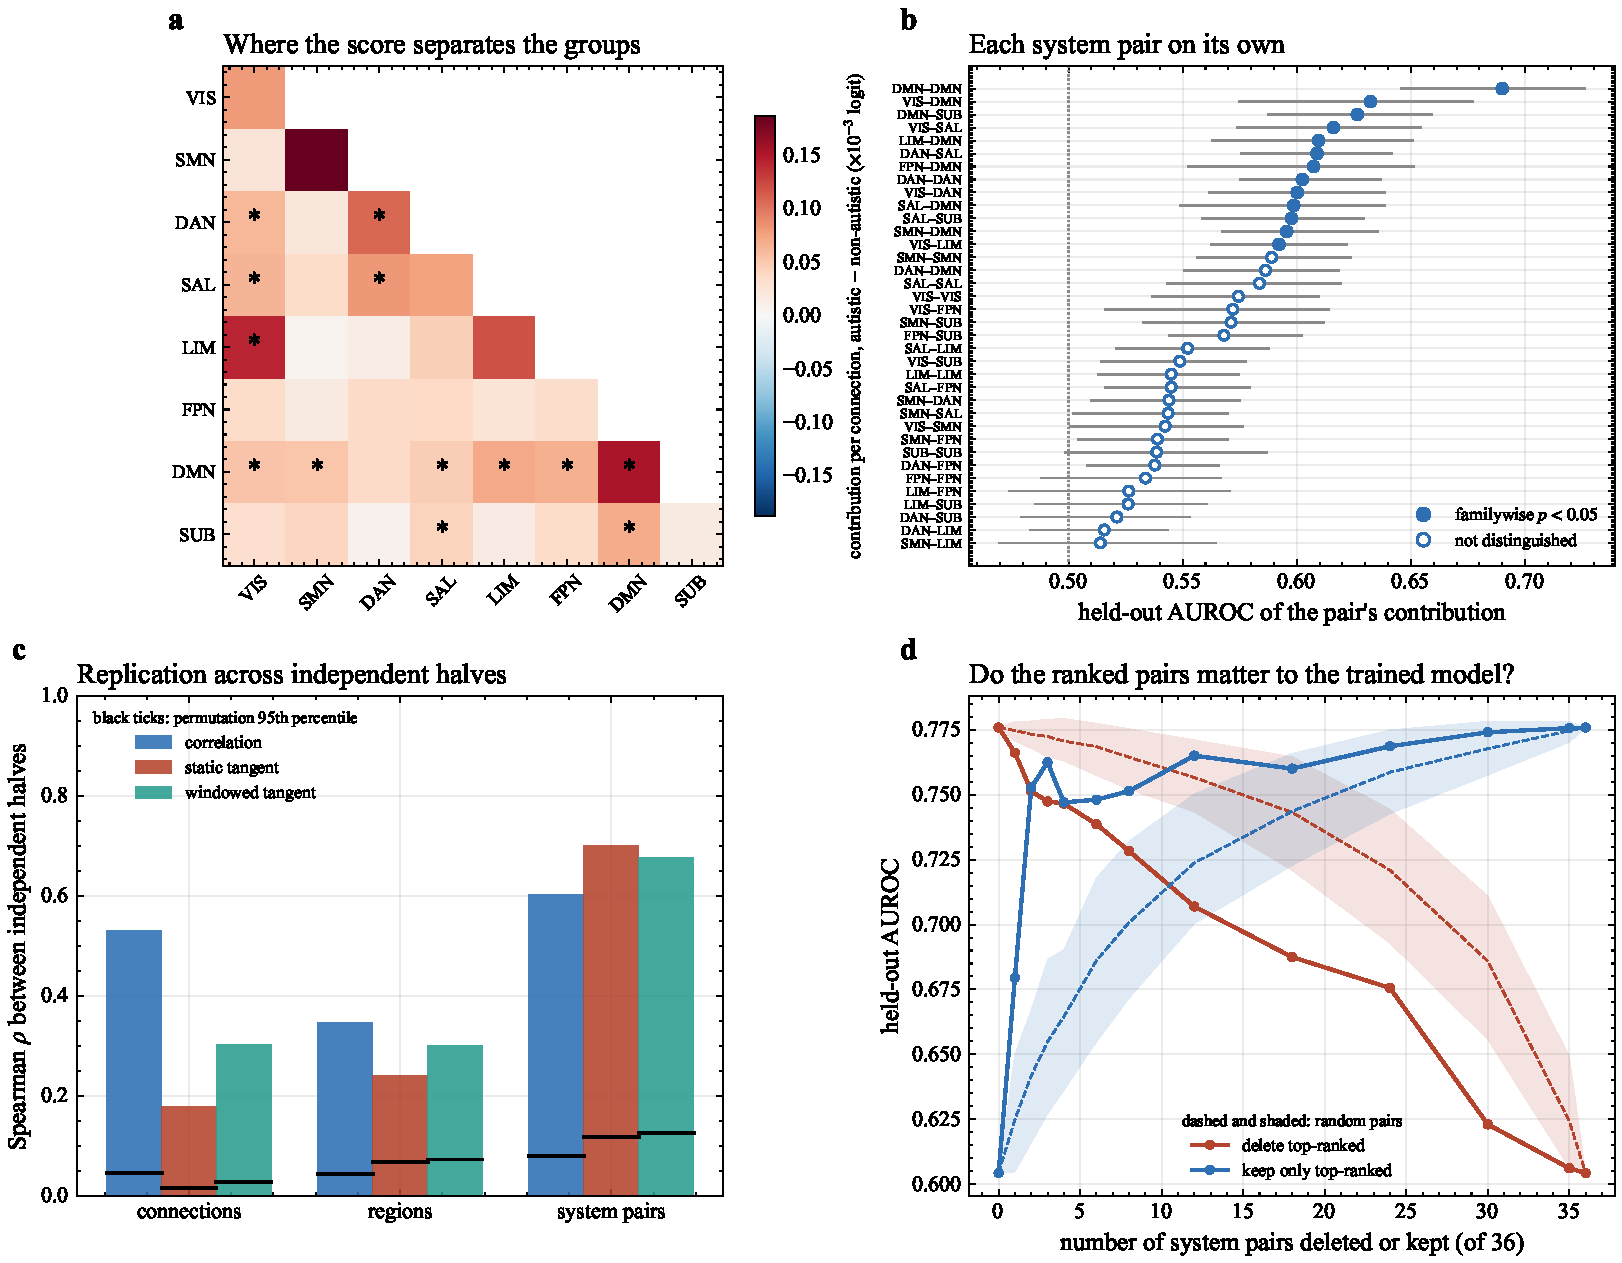
\includegraphics[width=\linewidth]{fig_interpretation}
\caption{Attribution of the ensemble score to functional-system pairs (system codes as in Figure~\ref{fig:overview}). (a) Between-group difference in mean contribution per connection, averaged across the three views and pooled held-out predictions; asterisks mark pairs whose held-out AUROC exceeds the permutation maximum (familywise $p<0.05$). (b) Held-out AUROC for each pair alone, with 95\% site-clustered bootstrap intervals; filled markers indicate familywise $p<0.05$. (c) Spearman correlation of structure coefficients between independent cohort halves for each view and level; black ticks show the 95th percentile under diagnosis permutation. (d) Held-out AUROC after the highest-ranked system pairs from the training fit are deleted or retained alone, compared with random pairs; the dashed line and shading show the random-pair mean and 95\% range.}
\label{fig:interpretation}
\end{figure}


System-pair attribution shows that default-mode connections contribute most to classifier separation. Within-default-mode connectivity accounts for 12.9\% of the total separation, followed by default mode--subcortical/cerebellar at 9.4\% and visual--default mode at 6.4\% (Table~\ref{tab:system-contributions}). Because contribution share is related to the number of connections in each pair ($\rho=0.72$), contributions are also examined per connection. On this scale, the largest effect occurs within the somatomotor system, followed by within-default-mode and visual--limbic connectivity. Individual system pairs provide only moderate discrimination on held-out participants; within-default-mode reaches an AUROC of 0.690, and 13 of 36 pairs exceed the familywise permutation reference (Figure~\ref{fig:interpretation}b).

Reproducibility is stronger at the system level than at finer anatomical scales. Across non-overlapping participant halves, system-pair structure coefficients correlate at 0.60, 0.70, and 0.68 for the correlation, static tangent, and windowed views, respectively, all above their permutation references (Table~\ref{tab:pattern-reproducibility}; Figure~\ref{fig:interpretation}c). Regional and connection-level agreement is weaker, and classifier weights are less reproducible than structure coefficients. Because these participant halves still contain data from all acquisition sites, a stricter site-disjoint analysis is also performed using 40 splits of the 20 sites into two non-overlapping groups (Section~\ref{subsubsec:site-disjoint}). System-pair agreement remains substantial at 0.54, 0.63, and 0.57 across the three views and remains above permutation references after adjustment for site indicators, age, sex, and mean FD. Agreement is positive in every site split, whereas individual-connection agreement remains lower. Together, these analyses support functional-system attribution as a more reproducible level of interpretation than individual connections.

\begin{table}[t]
\centering

\caption{Agreement between patterns fitted in two independent halves of the cohort, reported as the mean Spearman correlation across 40 random splits. For each connection, the structure coefficient is its correlation with the model score, and the weight is its model coefficient. Values in brackets show the 95th percentile obtained after within-site diagnosis permutation. Sign agreement is the percentage of connections, regions, or system pairs with the same structure-coefficient sign in both halves, with the permutation mean shown in brackets.}

\label{tab:pattern-reproducibility}
\small
\begin{tabular}{@{}llccc@{}}
\toprule
View & Level & Structure coefficients $\rho$ & Sign agreement (\%) & Weights $\rho$ \\
\midrule
Correlation & Connections & 0.530 (0.045) & 64 (51) & 0.152 (0.008) \\
 & Regions & 0.346 (0.044) & 47 (51) & 0.149 (0.024) \\
 & System pairs & 0.603 (0.080) & 64 (51) & 0.334 (0.049) \\
\midrule
Static tangent & Connections & 0.179 (0.015) & 56 (50) & 0.092 (0.005) \\
 & Regions & 0.240 (0.067) & 54 (53) & 0.128 (0.029) \\
 & System pairs & 0.701 (0.118) & 78 (55) & 0.547 (0.078) \\
\midrule
Windowed tangent, mean & Connections & 0.302 (0.028) & 60 (51) & 0.128 (0.006) \\
 & Regions & 0.301 (0.072) & 58 (53) & 0.141 (0.029) \\
 & System pairs & 0.676 (0.126) & 71 (55) & 0.442 (0.079) \\
\bottomrule
\end{tabular}
\end{table}


The three connectivity views show different levels of agreement. Static tangent and windowed connectivity are highly similar across the 36 system pairs (Spearman correlation 0.90), whereas the correlation view agrees less strongly with the static tangent and windowed views (0.55 and 0.64). The correlation view also aligns closely with the nuisance-adjusted system-level group differences, with correlations of 0.93 in the full cohort and 0.89 after motion matching. The corresponding values are lower for static tangent connectivity (0.43 and 0.58) and windowed connectivity (0.55 and 0.73). Within the somatomotor system, regional patterns agree strongly with the regional group differences in all three views (0.93, 0.79, and 0.78). Because the classifier itself is not adjusted for site, motion, age, or sex, this agreement is interpreted as descriptive rather than as a direct validation of the classifier. The highest-ranked system pairs also contribute meaningfully to held-out predictions (Figure~\ref{fig:interpretation}d). Removing the 12 highest-ranked pairs reduces AUROC from 0.776 to 0.707, compared with 0.757 for 12 randomly selected pairs (95\% range 0.743--0.771). Conversely, retaining only the 3 highest-ranked pairs, together with the unassigned connections, gives an AUROC of 0.763, compared with 0.655 for 3 random pairs. Similar patterns are observed under LOSO validation: AUROC falls to 0.710 after removing the highest-ranked pairs, compared with 0.756 for random removal, while retaining the highest-ranked pairs gives 0.749 compared with 0.648 for random retention. Because these analyses remove or retain features without refitting the model, they show which system pairs the trained classifier relies on rather than whether a newly fitted model could compensate for their absence. The information is nevertheless distributed across multiple pairs, as removing the 6 highest-ranked pairs lowers AUROC by only 0.037.

\subsection{Conditions for trustworthy use}
\label{subsec:results-trust}

Figure~\ref{fig:trust} examines three factors that determine whether the recalibrated probabilities remain reliable: the \reviewdel{site prevalence}\reviewhl{observed site autistic proportion}, the chosen operating point, and participant or site strata. Residual site-level calibration offsets are strongly associated with the autistic proportion of the withheld site (Spearman $\rho=0.79$; Figure~\ref{fig:trust}a). Adjusting the intercept to the true site proportion removes the observed heterogeneity, reducing $I^2$ from 63\% to 0\% and the mean absolute offset from 0.41 to 0.25. This analysis identifies variation in the \reviewdel{site prevalence}\reviewhl{site autistic proportion} as an important source of calibration shift, but it is not directly deployable because the true proportion is unknown at a new site. Figure~\ref{fig:trust}b shows that the correction is useful only when the \reviewdel{prevalence}\reviewhl{autistic proportion} is estimated accurately, approximately within 0.05. Estimation from unlabelled predictions performs poorly, while using 10 or 15 labelled participants reduces but does not remove the remaining heterogeneity. These results indicate that probability calibration at a new site depends on reasonably accurate knowledge of its \reviewdel{autistic prevalence}\reviewhl{autistic proportion}.

\reviewdel{Operating thresholds are more transferable than absolute probabilities.}\reviewhl{Participant-pooled operating-point performance is more stable than site-level probability calibration in these analyses.} Thresholds selected entirely from the training partition \reviewdel{achieve their intended sensitivity or specificity on held-out participants}\reviewhl{meet their predefined sensitivity or specificity target in participant-pooled held-out predictions under both validation protocols} (Figure~\ref{fig:trust}c). Under LOSO validation, the specificity-targeted rule reaches a specificity of 0.84, while the sensitivity-targeted rule reaches a sensitivity of 0.80. \addhl{Decision-curve analysis is a mathematical sensitivity analysis, because no clinical decision is defined for a positive classification in ABIDE-I. Relative to the better of treating all participants (at 0.30 and 0.40) and treating none (at 0.50), the recalibrated probabilities gain a net benefit of 0.05, 0.11, and 0.18 at threshold probabilities of 0.30, 0.40, and 0.50 under pooled validation, and of 0.05, 0.11, and 0.16 with a site withheld, with every 95\% site-clustered interval above zero (Figure~}\ref{fig:trust}\addhl{d).} Recalibration changes the interpretation of the probability scale but produces little change in net benefit. These operating-point results are specific to the present cohort, in which 46\% of participants are autistic. At lower \reviewdel{prevalences}\reviewhl{autistic proportions}, positive predictive value decreases substantially, so the findings support \reviewdel{transfer of decision thresholds across comparable research sites}\reviewhl{aggregate held-out operating-point performance within ABIDE-I} rather than population screening. \reviewhl{Site-specific target attainment was not established for every withheld site.}

Stratified analyses provide a further check on reliability across participant and site characteristics. AUROC does not differ detectably across age groups or thirds of head motion, as the intervals for differences between extreme strata include zero (Figure~\ref{fig:trust}e). Under LOSO validation, performance is lower at smaller sites, with AUROC 0.74 for sites with fewer than 40 participants compared with 0.82 for sites with at least 80 participants. After recalibration, no age, motion, or site-size stratum has a calibration offset whose interval excludes zero (Figure~\ref{fig:trust}f). Some residual differences remain in direction and magnitude, particularly across age groups, and these are not consistently explained by stratum prevalence. Together, these analyses show that discrimination is relatively stable across the examined participant strata, while probability calibration remains more sensitive to site composition and base rate.

\begin{figure}[pos=tbp]
\centering
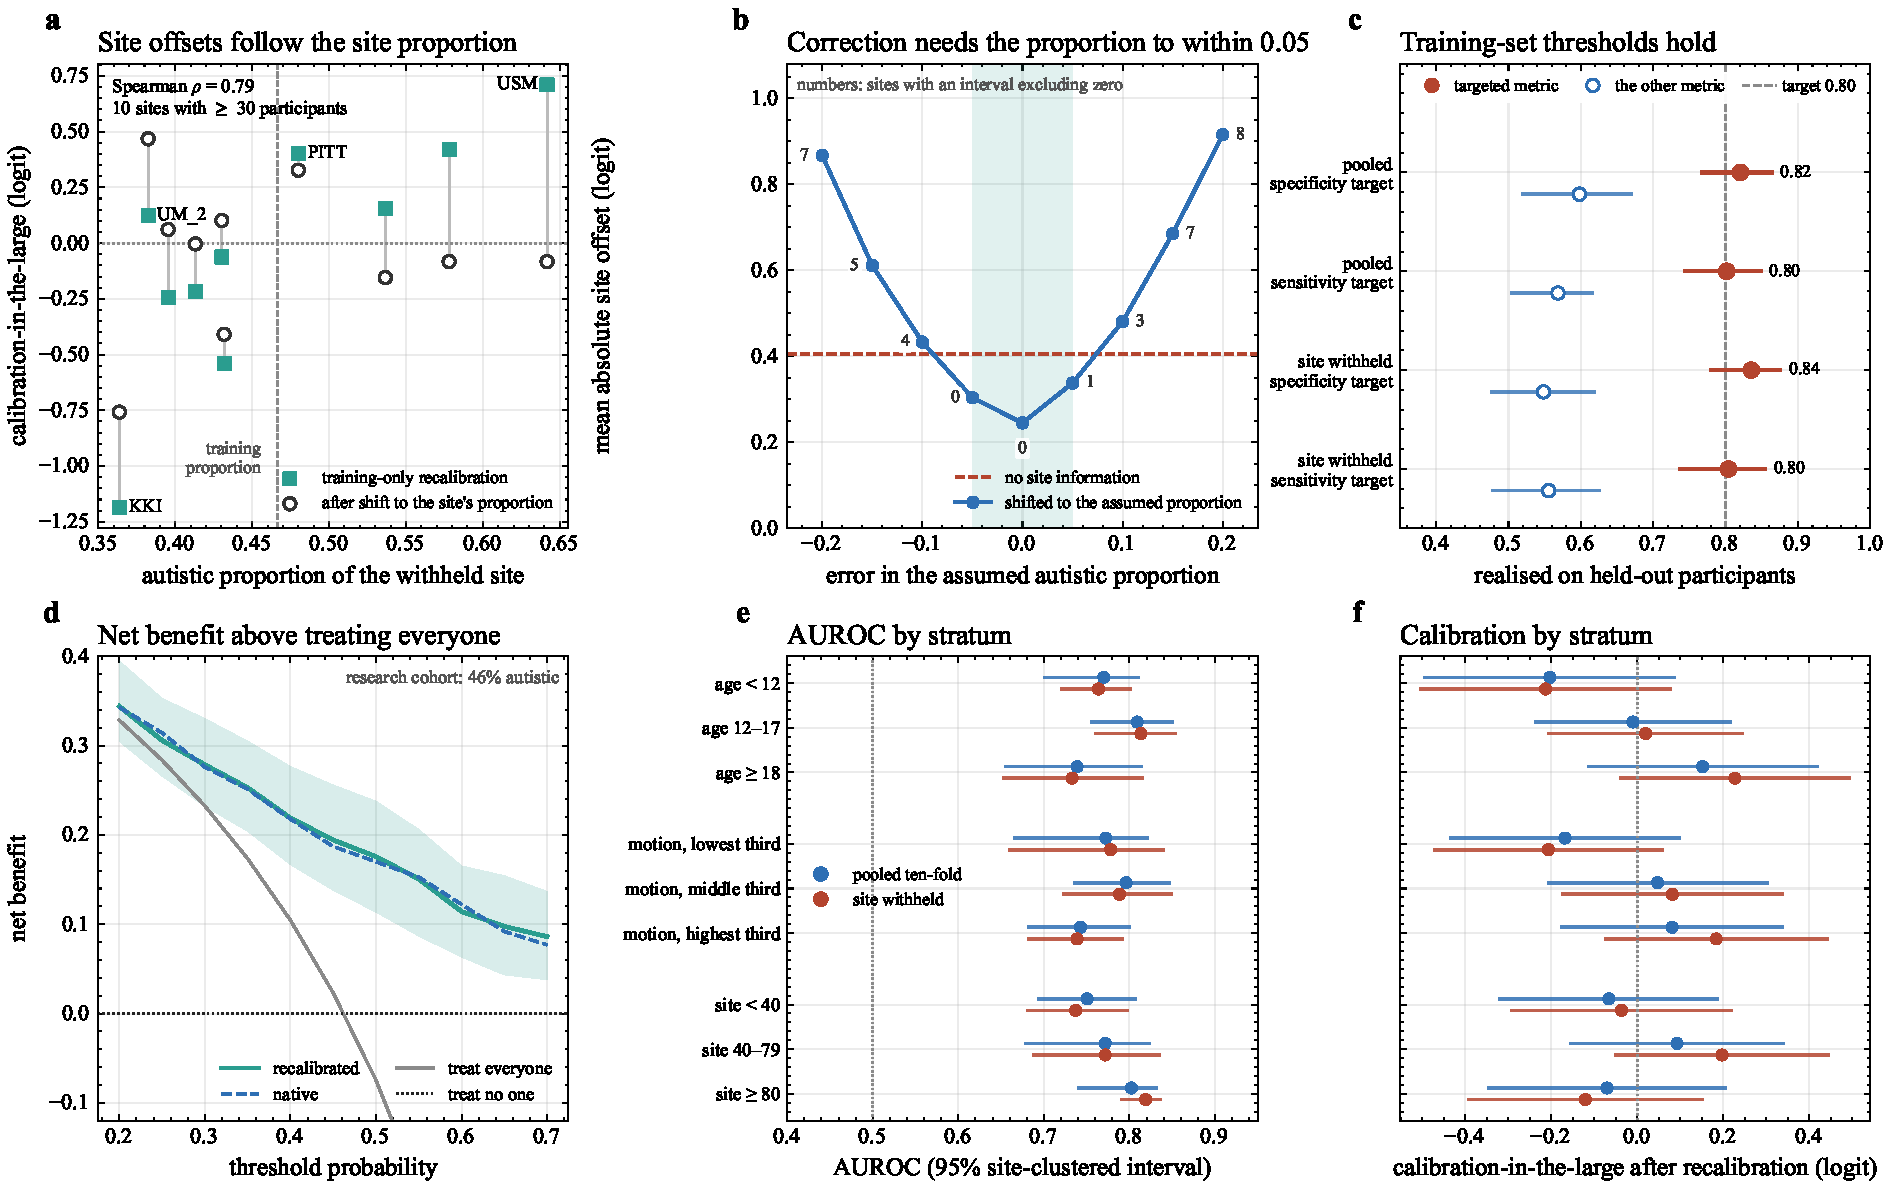
\includegraphics[width=\linewidth]{fig_trust}
\caption{Conditions for reliable use of recalibrated probabilities. (a) Residual site-level calibration offset in relation to autistic prevalence, before and after prevalence adjustment. (b) Sensitivity of calibration to error in the assumed site prevalence. (c) Sensitivity and specificity of thresholds selected from the training data and evaluated on held-out participants. (d) \addhl{Net benefit of native and recalibrated probabilities, with treating all participants and treating none as references.} (e) AUROC across age, motion, and site-size strata. (f) Calibration-in-the-large across the same strata after recalibration.}
\label{fig:trust}
\end{figure}

\subsection{Secondary results}
\label{subsec:results-secondary}

Three secondary analyses are reported in the Supplementary Material and are not treated as study contributions. Confidence-based abstention provides no useful guarantee: the cohort-wide rule meets its target in 0.816 of 38 valid half-splits against a nominal 0.90, and the per-site rule meets it in 0.914 of 197 only while answering 13.7\% of participants. Combining CC200 with anatomical atlases does not improve discrimination (fold-mean AUROC 0.749--0.755 against 0.756 for CC200 alone). A label-noise sensitivity analysis cannot identify the accuracy attainable against the diagnostic labels because its assumptions are not supported by the data.
